%\documentstyle[epsf,twocolumn]{jarticle}       %LaTeX2.09仕様
%\documentclass[twocolumn]{jarticle}     %pLaTeX2e仕様
\documentclass[twocolumn]{jarticle}     %pLaTeX2e仕様

%一枚組だったら[twocolumn]関係のとこ消す

\setlength{\topmargin}{-45pt}
%\setlength{\oddsidemargin}{0cm} 
\setlength{\oddsidemargin}{-7.5mm}
%\setlength{\evensidemargin}{0cm} 
\setlength{\textheight}{24.1cm}
%setlength{\textheight}{25cm} 
\setlength{\textwidth}{17.4cm}
%\setlength{\textwidth}{172mm} 
\setlength{\columnsep}{11mm}

\kanjiskip=.07zw plus.5pt minus.5pt

\usepackage{graphicx}
\usepackage[dvipdfmx]{color}
\usepackage{subcaption}
\usepackage{enumerate}
\usepackage{comment}
\usepackage{url}
\usepackage{multirow}
\usepackage{diagbox}
\usepackage{amsmath,amssymb}
\usepackage{mathtools}
\usepackage{wrapfig}
\usepackage{graphicx}
\usepackage{float}
\usepackage{algorithmic}
\usepackage{algorithm}

\begin{document}
\twocolumn[
  \noindent
  \hspace{1em}

  情報工学英語演習
  \hfill
  \ \  学籍番号1201201100 西村昭賢 

  \vspace{2mm}
  \hrule
  \begin{center}
  {\Large \bf Gradient-Based Learning Applied to Document Recognition の要約}
  \end{center}
  \hrule
  \vspace{3mm}
]

\section*{著者}
Yann LeCun, L\'{e}on Bottou, Yoshua Bengio, and Patrick Haffner \cite{thispaper}

\section*{概説}
逆伝搬法で学習した多層ニューラルネットワークは,勾配に基づく学習法の最たる成功例である.適切なネットワークアーキテクチャがあれば,勾配に基づく学習アルゴリズムは分類可能な複雑な決定超平面を,最小限の前処理で 作成することができる.本論文では,手書き文字の認識に適用される様々な方法を振り返り,標準的な手書き整数認識タスクを用いて比較する.その結果, CNN が他の手法に比べて良い性能を示した.
\par
実際の文章認識システムは,複数のモジュールにより構成されている. Graph Transformer Networks (GTN) と呼ばれる新しい学習の枠組みにより,このような多くのモジュールからなるシステムを勾配に基づく学習アルゴリズムを用いて大域的に学習することが可能となった.
\par
本論文では,オンライン手書き文字認識の 2 つのシステムを紹介する.
実験により,大域的な学習の利点と GTN の柔軟性が示された.
\par
また,本論文では銀行小切手を読み取るGTNも紹介する. この手法は, 
商業的に利用されており,1日あたりに数百万の小切手の認識をしている.
\par
キーワード -- ニューラルネットワーク, OCR, 文章認識, 機械学習, 勾配に基づく学習, CNN, Graph Transformer Networks, Finite State Tranducers.

\section*{略称}
\begin{quote}
  \begin{itemize}
   \item GT Graph transformer
   \item GTN Graph transformer network.
   \item HMM Hidden Markov model.
   \item HOS Heuristic oversegmentation
   \item K-NN K-nearest neighbor
   \item NN Neural network.
   \item OCR Optical character recoginiton.
   \item PCA Principal component analysis.
   \item RBF Radial basis function.
   \item RS-SVM Reduced-set support vector method.
   \item SDNN Space displacement neural network.
   \item SVM Support vector method.
   \item TDNN Time delay neural network.
   \item V-SVM Virtual support vector method.
  \end{itemize}
 \end{quote}

 \section{序論}

ここ数年, パターン認識システムの設計において, ニューラルネットワークが非常に重要な役割を果たしている. 
実際に,近年の音声認識,手書き文字認識といったパターン認識アプリケーションの成功にはこのような学習法の利用が重要な要因であると言える.\par
本論文の主な主張は,人間の経験的な知識に頼らず自動的な学習に依存して, より良いパターン認識システムを作成することができるということだ.
これは,近年の機械学習や情報工学の進歩により可能となった.
本論文ではこれまでの手作業の特徴抽出が, 学習機械に置き換えることができることを示している.また文章認識を例として,本論文では個々に設計されたモジュールを組み合わせることで認識システムを作る従来の方法を,全てのモジュールを学習するGTNと呼ばれる枠組みに置き換えることができることを示している.
\par
パターン認識の研究初期から,手作業で完全に正確なパターン認識システムを作成することは難しいことが知られている. そのため多くのパターン認識システムは自動的な学習と人間が考案したアルゴリズムを組み合わせて作られている. パターンを認識するための一般的な方法は, システムを特徴抽出器と分類器の 2 つの主なモジュールに分けて構成することである.
特徴抽出器では入力パターンを, (a)照合・比較しやすく,(b)入力パターンの変形や歪みに対して比較的頑強である低次元のベクトルや短い配列で表現できるように変形する .特徴抽出器はタスクに特化しており, ほとんど手作業で作られるため,設計の際の作業の大半を占める.
もう一方は分類機と呼ばれるモジュールであり,汎用的で学習可能である.
このアプローチの大きな問題の1つは, 設計者によって認識精度が大きく依存することだ.\par
これまでは, 分類器が用いる学習方法がクラス分類可能な低次元空間に限定されていたため特徴抽出器が必要とされた. しかし, この10年間で3つの要因が重なりこの見解は変化してきた.
1つ目の要因は計算機の性能向上, 2つ目の要因は大規模なデータベースが使用可能になり実データに依存した認識器の設計が可能になったこと, 3つ目の要因は高性能な機械学習方法が生み出されたことである. 近年の音声認識や手書き文字認識システムの精度向上には, これらの要因が大きくかかわっている.
\par
本論文では手書き文字認識における課題点を検討し (1 章, 2 章), 手書き数字データセットにおいていくつかの学習方法の性能を比較した (3 章). 2 章で紹介する CNNは, 2次元形状の不変性に対する予備知識を取り入れた特殊なニューラルネットワークの1つである. 分離された手書き整数認識タスクに対するいくつかの方法の比較を 3 章で示す. 4 章では全体の誤差を減らすため学習した多くのモジュールを組み合わせる GTN の方法を紹介する. 5 章では, 古典的なヒューリスティックなオーバーセグメンテーションを紹介する. 6章では手動の前処理を必要としない単語レベルでの識別機の学習を可能にするような識別的,非識別的な勾配に基づく学習法を紹介する. 7 章では, 入力における全ての位置において認識器を作用させる空間置換ニューラルネットワークのアプローチを示す.
8 章では, 学習可能なGTNが一般的なグラフ構成アルゴリズムに基づく複数の一般化変換として定式化できることを示している.
また, HMM と GTN の関連も示す.
9 章は,ペン型コンピュータで入力された手書き文字を認識するための大域的に学習されたGTNシステムについて説明する.
計算機が即座に応答を返さなければならないため, この問題は"オンライン"手書き文字認識として知られている. GTNシステムの中核はCNNである. 本研究で得られた結果は, 文字レベルではなく単語レベルで学習することの利点を示している.
10 章は, 銀行小切手を認識する GTN に基づいた完全なシステムを説明する. このシステムの中核は 2 章で述べる LeNet-5 と呼ばれる CNN である.

\subsection*{A. データからの学習}
機械学習を自動化するためのアプローチとして, 最も成功を収めた 1 つは,勾配に基づく学習と呼ばれるアプローチである.
学習する計算機は関数 $Y^p = F(Z^p,W)$ を計算する.ここで, $Z^p$ は $p$ 番目の入力パターンであり, $W$ はシステムにおける調整可能なパラメータの集合を表す.
パターン認識の設定では, 出力 $Y^p$ はパターン $Z^p$ の認識可能なクラスラベル,あるいは各クラスに関係する確率やスコアとして解釈できる.損失関数 $E^p = \mathcal{D}(D^p,F(W,Z^p))$ は, パターン $Z^p$ における望ましい出力 $D^p$ とシステムの出力との不一致さを測定する.平均損失関数 $E_{train}(W)$ は学習データセット {($Z^1$,$D^1$),...,($Z^P$,$D^P$)} と呼ばれるラベル付きの学習データの集合上の誤差 $E^p$ の平均値である.
最も単純な設定において,学習問題は$E_{train}(W)$を最小化する$W$の値を見つけることである.実際には, テストデータと呼ばれる学習データセットとは異なるデータセットを用いて性能を評価することが重要である.多くの理論的・実験的研究により,テストデータで予測されるエラー率と学習データで期待されるエラー率との間の差は学習データ数によっておおよそ式 \ref{式1} のように減少することが分かっている. 

\begin{equation}
  E_{test} - E_{train} = k({h}/{P})^\alpha
  \label{式1}
\end{equation}
ここで $P$ は学習データ数であり, 
$h$ は「有効容量」,機械の複雑さの推定値, $\alpha$ は 0.5 ~ 1.0 の値で, $k$ は定数である.学習サンプルの数が増加した時は差は常に減少する.その上 $h$ が増加すると, $E_{train}$ が減少する.従って, $h$ が増えた時, 最小の汎化誤差 $E_{test}$ を達成する容量 $h$ の最適な値があれば,$E_{train}$ の減少量と差の増加はトレードオフの関係となる.
多くの学習アルゴリズムは $E_{train}$ だけでなく差の増加も最小化しようと試みる. 実際には $E_{train} + \beta H(W)$を最小化することを意味している.ここで関数 $H(W)$ は正規化関数と呼ばれ, $\beta$ は定数である. $H(W)$はパラメータ空間の部分集合に所属するパラメータ $W$ に関して大きな値を取るように選択される. $H(W)$ を最小化することで,パラメータ空間におけるアクセス可能な部分集合の容量を制限する.それにより学習データにおける誤差の最小化と学習データとテストデータの誤差の差の最小化のトレードオフを制御する.

\subsection*{B. 勾配に基づく学習}
パラメータ集合に関する関数の最小化は,コンピュータサイエンスにおける多くの問題の根底となっている. 勾配に基づく学習は
,一般的に離散関数よりも滑らかな連続関数を最小化するほうがはるかに簡単という事実に基づいている.
損失関数はパラメータの値の変動が及ぼす影響を推定することで最小化できる.この推定はパラメータに対する損失関数の勾配によって行われる. 分析的に勾配ベクトルが計算できるようになると効率的な学習アルゴリズムが考案されうる.このことが連続値のパラメータを持つ多くの勾配に基づく学習アルゴリズムの基礎となっている.
本論文で示す手順では,
パラメータ集合 $W$ は実数値のベクトルであり $E(W)$ は連続であり,ほぼ全て微分可能である.このような問題設定における最も単純な最小化の手順は勾配降下法であり $W$ は式 \ref{式2}のように再帰的に調整される.

\begin{equation}
  \label{式2}
  W_{k} = W_{k-1} - \epsilon \frac{\partial E(W)}{\partial W}
\end{equation}

もっとも簡単なケースでは $\epsilon$ は定数である. より洗練された手順では変数として $\epsilon$ を用いるか, $\epsilon$ を対角行列に置き換えるか, Newton 法や Quasi-Newton 法のようにヘッシアン行列の逆行列の推定値に置き換える. 共役勾配法も用いられる.
\par
一般的な最小化手法はオンライン更新とも呼ばれる確率的勾配アルゴリズムがある.
これは勾配平均のノイズを含んだもの, 近似したものを用いてパラメータのベクトルを更新する手法である. 
\begin{equation}
  \label{式3}
  W_{k} = W_{k-1} - \epsilon \frac{\partial E^{p_k}(W)}{\partial W}
\end{equation}
この手順では, パラメータベクトルは平均の系列を中心に変動する.しかし, 通常の勾配降下法や2次元の勾配アルゴリズムに比べて冗長な大規模な学習データにおいてはかなり高速に収束する. 
このようなアルゴリズムの学習への応用は1960年代から理論的に研究されていた. しかし, 80 年代半ばまでは非自明な問題に対する実用的な成功例は起こっていなかった.

\subsection*{C . 勾配逆伝搬法}
勾配に基づく学習法は 1950年代後半から用いられていたが, 複雑な機械学習タスクに対する単純な勾配降下法の驚くべき有用性は以下の 3 つの出来事が起こるまで広く知られていなかった.
 1 つ目は損失関数の局所的最小値が実際には大きな問題にならないことが認識されたことである. これはボルツマンマシンといった非線形の勾配に基づく学習の成功において局所的最小値が大きな障害になっていないと考えられたことで認識された.
 2 つ目の出来事は数層の処理からなる非線形システムにおける勾配を計算するための逆伝搬法が一般化されたことである. 3 つ目の出来事はシグモイド関数を有したユニットからなる多層ニューラルネットワークに逆伝搬法を適用することで複雑な学習タスクを解決できることが示されたことである.
 逆伝搬法の基本的なアイデアは出力から入力への伝搬により勾配を効率的に計算することである. このアイデアは 60 年代初期に考えられていたが, 機械学習への応用は一般に認識されていなかった.興味深いことに, 深層学習の文脈における初期の逆伝搬法の導出は, 勾配ではなく「仮想ターゲット」を用いていた.
 制御理論の文献で用いられていたラグランジュ形式は, 逆伝搬法やRNN, 異種のモジュールからなるネットワークへの逆伝搬法の一般化の導出においておそらく最も厳密な方法を提供した.
\par
多層ニューラルネットワークで局所最小値が問題にならないという事実は理論的には謎である. 
タスクに対してネットワークが大きすぎる場合, パラメータ空間の「追加の次元」の存在が到達不可能な領域の危険性を減らしていると推測されている.
逆伝搬法は, ニューラルネットワークの学習アルゴリズムとして最も広く用いられており, あらゆる形式の学習アルゴリズムで広く用いられている.

\subsection*{D. 手書き文字認識システムにおける学習}
分離された手書き文字の認識は 
ニューラルネットワークの初期の応用において最も成功した例の一つである. 手書き数字認識における比較実験では, 同じデータに対して, 勾配に基づく学習アルゴリズムを用いて学習したニューラルネットワークが他のすべての手法よりも優れた結果を記録した. CNN と呼ばれる最も優れたニューラルネットワークは画像から直接関連する特徴を抽出するために学習するように設計されている.\par
手書き文字の認識において最も困難な問題の 1 つは認識ではなくセグメンテーションとして知られる, 単語や文中から文字を分離する処理である.
分割のための技術として「ヒューリスティックオーバーセグメンテーション」と呼ばれる手法が一般的である.
この手法では, ヒューリスティックな画像処理手法により多数の文字間の切れ目の候補を作成し, その後認識器により最適な切れ目の候補の組み合わせを見つける. このようなモデルでは, システムの精度は作成された切れ目の候補の質と, 認識器が文字, 複数文字, 非文字と区別する能力に依存する.  このタスクを実行するための認識器の学習は, ラベル付きデータセットを作成することが困難であるため難題となっている.
文字列の画像を分割器に通して, すべての文字候補に手動でラベリングすることがもっとも簡単と考えられるが, この作業は非常に面倒で労力がかかるだけでなく, 一貫したラベリングが困難という問題も有している.
\par
5 章で述べる 1 つ目の解決策は, 文字列全体のレベルでシステムを学習させることである. このアイデアには勾配に基づいた学習の概念を使用することができる. このシステムは誤答の可能性を示す誤差関数の値を最小化するように学習を行う. 第 5 章では誤差関数が微分可能であり, 勾配に基づく学習方法に適しているということを調査する.
また, 枝が数値情報を持つ有向非巡回グラフの利用を紹介し GTN の概念を紹介する.
\par
7 章で述べる 2 つ目の解決策は, そもそも分割しないことである.このアイデアでは, 入力画像上の可能なすべての位置に識別器を置き, 認識器の入力画像内に他の文字があっても中心にある文字を正しく認識できる機能に頼る.
そうして得られた認識器の出力の系列は,言語的制約を考慮に入れて最終的に最もらしい解釈を抽出する GTN に送られる. この GTN は隠れマルコフモデルに類似している.  この解決策はCNNを用いることでその特性により計算のコストを遥かに節約できるため特に魅力的である.

\subsection*{E. 大域的に学習可能なシステム}

 実用的なパターン認識システムは複数のモジュールから構成される.
ほとんどの場合, モジュール間で伝搬する情報は枝に数値が付与された非巡回グラフとして表現されるのが最適である. 典型的には各モジュールは手動で最適化されるが, 時には認識システムの流れから独立して学習される.この手動で調整する段階は非常に面倒であり時間がかかり, さらにはほとんどの場合確実に最適とは言えない.
\par
よりよい代替案として, 大域的な誤差を最小化するようにシステム全体を学習させることである.理想的にはシステムのすべてのパラメータについて大域的な損失関数の最小値を見つけたい. もしシステムの性能を測定する損失関数 $E$ がシステム内の調整可能なパラメータ $W$ に対して微分可能であれば, 勾配に基づく学習により損失関数 $E$ の局所的最小値を求めることができる.
\par
大域的な損失関数 $E^p (Z^p , W)$ が微分可能であることを保証するために, システム全体は微分可能なモジュールの FFN として構成されている. 各モジュールにより実装される関数は, モジュールのパラメータとモジュールの入力に対して連続的であり, かつほとんどの場所で微分可能である必要がある.
この場合, 良く知られている逆伝搬法の単純な一般化を用いてシステムの全てのパラメータに対する損失関数の勾配を効率的に計算することができる.
例えば,  システムがモジュールの連鎖として構成されていると考えると,関数 $X_n = F_n (W_n , X_{n-1})$ として解釈される.
ここで, $X_n$ はモジュールの出力を表すベクトル, $W_n$ はモジュールの調整可能なパラメータのベクトル ($W$ の部分集合) , $X_{n-1}$ はモジュールの入力ベクトル (直前のモジュールの出力ベクトル) である.
最初のモジュールの入力 $X_0$ は, パターン系列 $Z^p$ である. $X_n$ に関する $E^p$ の偏導関数が既知であれば, 後退型回帰を用いて, $W_n$ と $X_{n-1}$ に関する $E^p$ の偏導関数を計算することができる.
\begin{eqnarray}
  \frac{\partial E^p}{\partial W_n} = \frac{\partial F}{\partial W} (W_n , X_{n-1}) \frac{\partial E^p}{\partial X_n}  \nonumber \\ 
  \frac{\partial E^p}{\partial X_{n-1}} = \frac{\partial F}{\partial X} (W_n , X_{n-1}) \frac{\partial E^p}{\partial X_n} 
\end{eqnarray}
ここで, $\frac{\partial F}{\partial W} (W_n , X_{n-1})$ は $(W_n , X_{n-1})$ において評価された $W$ に関する $F$ のヤコビアン, $\frac{\partial F}{\partial X} (W_n , X_{n-1})$ は $X$ に関する $F$ のヤコビアンである. ベクトル関数のヤコビアンはすべての入力に関するすべての出力の偏導関数を含んだ行列である. 1 つめの数式は $E^p (W)$ の勾配を計算し, 2 番目の式は良く知られているニューラルネットワークにおける逆伝搬法の手順のように後退型回帰を計算する. 学習パターンに沿って計算された勾配を平均化すると, 完全な勾配を得ることができる.
上で示した式はヤコビアンと偏微分のベクトルの積を用いるが, ヤコビアンを前もって直接計算するよりもこの積を直接計算する方が簡単なことが多い. 一般的な多層ニューラルネットワークネットワークとの類似性から, 最後のモジュール以外のすべてのモジュールは出力が外部から観測できないため隠れ層と呼ばれる. 上で述べた単純に連結されたモジュール群に比べてより複雑な場合は, 偏微分の表記が曖昧なものとなる. また, 一般的な場合においての完全に厳密な導出はラグランジュ関数を用いて行われる.
\par
前に述べた通り, 複雑な認識システムにおける状態情報は枝に数値情報が付与された非巡回グラフで表現されることが最もである. このような場合, グラフ変換器と呼ばれる各モジュールは, 1 つかそれ以上のグラフを入力として, 出力として 1 つのグラフを生成する. このようなモジュールのネットワークを GTN と呼ぶ. 4, 6, 8 章では GTN の概念を発展し勾配に基づく学習を用いて大域的な損失関数を最小化するようにすべてのモジュール内のパラメータを学習できることを示す. 状態情報がグラフのような本質的に離散的なデータ構造で表現されるときに, 勾配が計算できるのは不可能に思えるが, この問題は後に示す通り回避できる.

\section{分離された文字認識への畳み込みニューラルネットワーク}
勾配降下法により学習された多層ネットワークは, 大量の教師データから複雑な高次元非線形マッピングを学習できるため, 画像タスクに向いている.
これまでのパターン認識のモデルでは, 手作業で設計された特徴抽出器で入力から関連する情報を集め無関係な変数を除去し, 学習可能な分類器で得られた特徴ベクトルをクラスに分類する. 
この手法では, 分類器として標準的な完全連結型多層ネットワークが用いられる. 
より興味深い手法は特徴抽出を可能な限り学習に頼ることである. 文字認識の場合, ネットワークはサイズ正規化された画像のようなほぼ前処理されていない画像を与えられる. 完全連結 FFN を用いることで文字認識などのタスクでいくつかの成功を収めているが, 問題点もある.
\par
第 1 に, 一般的な画像は数百もの変数 (画素値) を持つ大きなデータである. 例えば 100 個の隠れ層を持つ完全連結多層ネットワークの第 1 層は, 数万個の重みが含まれる. このような多数のパラメータによりシステムの規模が増加し, より大規模な学習データを必要とする. 
また, メモリに多くの重みを記録しておく必要があるため, 計算機の性能も求められる. しかし, 画像や音声アプリケーションへの非構造化ネットワークの主な欠点として入力の変換や局所的な歪みに対しての頑健性が組み込まれていない.
ニューラルネットワークの入力層に固定長のベクトルを渡す場合は, 文字画像や他の 2D, 1D 信号はサイズが正規化され入力領域の真ん中に置かれなければならない.
しかし, このような前処理を完璧に行うことはできない. 手書き文字はそれぞれの文字に対してサイズや傾き, 位置の相違が生じる. さらに書き方の違いまで組み合わさると, 入力における特徴的な位置にばらつきが生じる. 
原理的には, このようなばらつきに対して十分な大きさの完全連結ネットワークを用いることで対応する出力を生成するように学習できる. しかし, そのような学習では, 入力領域の特徴を検出するために入力の様々な位置に類似の重みパターンを持つ複数のユニットが配置されることになり, 結果として非常に多くの学習データが必要になる. 
\par
2 つ目の問題点として, 完全連結ネットワークのアーキテクチャにおいて, 入力のトポロジーが完全に無視されることである. 画像 (あるいは, 音声の時間周波数表現) には空間的, 時間的に近接した変数が高い相関を持つという強い 2 次元局所的構造を有する. この局所的な相関は, 空間的であれ時間的であれ認識対象を認識する前に局所的な特徴を抽出できる利点として良く知られている. しかし, 入力のトポロジーが無視されるためこの利点を生かすことができない. 

\subsection*{A. 畳み込みネットワーク}
畳み込みネットワークは, ある程度のずれ, 拡大縮小, 歪みの不変性を確保するために局所的受信可能領域, 重みの複製 , 時間的または空間的サブサンプリング の 3 つのアイデアをアーキテクチャに取り入れた. 図 \ref{fig:LeNet-5} に代表的な 文字認識のための CNN である LeNet-5 のアーキテクチャを示す.
\begin{figure}[t]
  \centering
  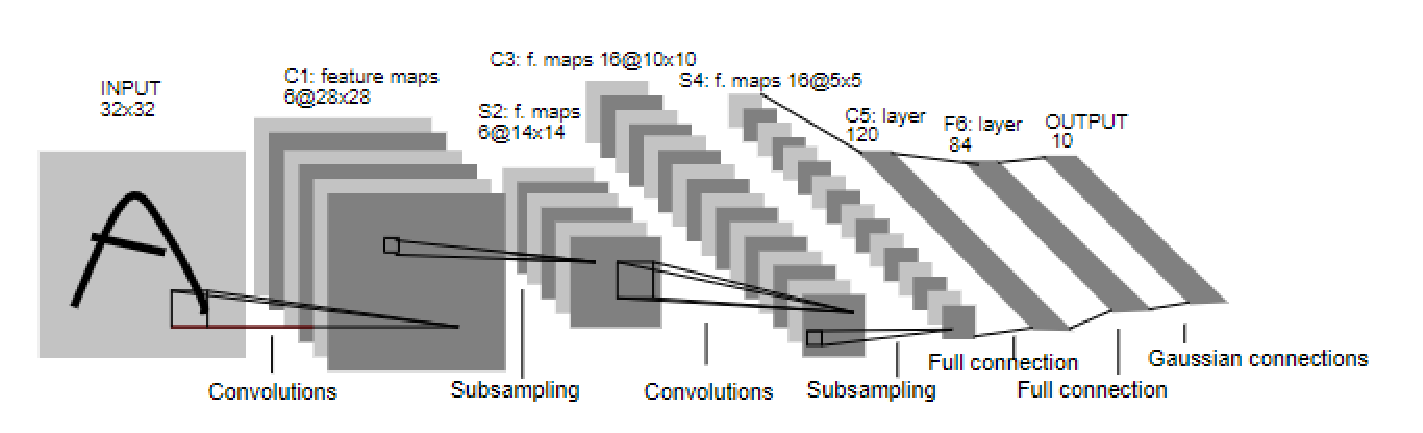
\includegraphics[width=80mm]{assets/2.eps}
  \caption{LeNet-5 のアーキテクチャ}
  \label{fig:LeNet-5}
\end{figure}

 畳み込みネットワークの入力では, おおよそサイズが正規化され文字が中央に配置された画像を入力する. 層の各ユニットは直前の層の小規模な近傍に位置するユニット群から入力を受け取る. 入力の局所的受信可能領域にユニットを接続するアイデアは, 60 年代初頭にすでに誕生していた.
局所的受信可能領域を持つニューロンは, 向きのあるエッジ, 終点, 角 といった様々な簡単な視覚的特徴を抽出することができ, これらの特徴はより高次の特徴を抽出するために後続する層によって結合される. 入力の歪みやずれにより重要度の高い特徴の位置が変化する場合があり, それに加えて画像の一部分で有効な特徴検出器は画像全体においても有効である可能性が高い. この知見は, 画像上の異なる場所に受信可能領域を持つユニットの集合に同一の重みベクトルをもたせることで応用できる.
層の中のユニットは, すべてのユニットが同じ重みの組を共有する平面で構成される. この平面におけるユニットの出力の集合を特徴マップと呼ぶ. 特徴マップのユニットはすべて画像の異なる部分に対して同じ動作をするよう制限されている. 完全な畳み込み層はいくつかの特徴マップから構成され, それぞれの位置において多くの特徴を抽出できる. 最初の隠れ層のユニットは 6 つの特徴マップで構成される. 
特徴マップのユニットは 25 個の入力を持ち, 入力の 5 × 5 の領域をユニットの受信可能領域と呼ぶ. それぞれのユニットは 25 個の入力を持つため, 結果として 25 個の学習可能な係数と学習可能な 1 つのバイアスを持つ. 特徴マップにおいて連続するユニットの受信可能領域は, 直前の層の対応するユニットの中央に配置される.
そのため, 隣接するユニットの受信可能領域は重なり合う. 先述したように, 1 つの特徴マップ内のすべてのユニットは, 同じ重みとバイアスを共有するため入力上の可能なすべての位置において同じ特徴を検出可能である.
層内の同じ特徴マップは異なる重みとバイアスを用いており, 異なる種類の局所的特徴を抽出する. 特徴マップの逐次的な解釈により, 局所的受信可能領域を持つ 1 つのユニットから入力画像を精査し, そのユニットの状態を特徴マップの対応する位置に格納する. 
この操作が畳み込みとそれに付随する加算バイアスおよび活性化関数に相当するため, 畳み込みネットワークと呼ばれている.
 特徴マップのユニットにより用いられる接続の重みの集合が畳み込みのカーネルである. 畳み込み層では, 入力画像にずれが生じると, 特徴マップの出力も同程度ずれ, それ以外は変更されない特性があり, この特性は, 入力の歪みやずれに対しての CNN の頑健性の基礎となる.
\par
他の特徴量とのおおよその相対的な位置のみが重要であるため, 一度特徴が検出されると, その抽出個所の位置はあまり重要ではなくなる. 絶対的な位置はパターン認識において無関係だけでなく, 精度を落とす要因になる可能性もある.
特徴マップの空間解像度を下げることで, 簡潔に特徴マップの中で識別可能な特徴量の位置の精度を減少させることができる. これはいわゆるサブサンプリング層で実現でき, 特徴マップの解像度を下げることでずれや歪みへの出力の感度を下げることができる.
LeNet-5 の 2 つ目の隠れ層はこのサブサンプリング層である. この層は 6 つの特徴マップからなり, 各特徴マップそれぞれは前の層の特徴マップに対応している. それぞれの特徴マップにおける受信可能領域は前の層の特徴マップの 2 × 2 の領域である. 各ユニットは 4 つの出力の平均を計算し, 学習可能な係数を乗算し, 学習可能なバイアスを加算し, 結果をシグモイド関数に渡す. 連続するユニットは重なりがない連続した受信可能領域を持つ. その結果, サブサンプリング層の特徴マップは行と列の数が半減する. 学習可能な係数とバイアスは, シグモイドの非線形性の度合いを制御する.
サブサンプリング層と畳み込み層の繰り返しは, 一般的には交互に起こる. 各層において, 特徴マップの数は空間解像度が減少するにつれ増加する. 図 \ref{fig:LeNet-5} の 3 つ目の隠れ層のそれぞれのユニットは, 直前の層のいくつかの特徴マップからの入力接続を持つ.
表現の豊かさ (特徴マップの数) を徐々に増加させ, 空間解像度を徐々に減らすことで, 入力の幾何学的変換に対して高い不変性を持たせることが可能である.
\par 
すべての重みは逆伝搬法により学習されるため, 畳み込みネットワークは自身の特徴抽出器を合成しているとみなすことができる. 重みの複製技術は, パラメータを減らすという興味深い効果を持ち, それにより学習時のエラーとテスト時のエラーの差を減らすことができる. 図 \ref{fig:LeNet-5} のネットワークは 340908 個の接続を持つが, 重みの複製により学習可能な自由パラメータは 60000 個である.
\par
固定されたサイズの畳み込みネットワークは手書き文字, 機械印刷文字, オンライン手書き文字, 顔 など様々な認識アプリケーションに採用されてきた. 
 \subsection*{B. LeNet-5}
 本章では, 実験で用いた CNN である LeNet-5 のアーキテクチャをより詳細に説明する.
  LeNet-5 は入力層を除く 7 層から構成され, それらすべての学習可能なパラメータが設定されている. 入力は 32 × 32 ピクセルの画像である. これはストロークの終点や角といった潜在的な特徴量が特徴抽出器の受信可能領域の中心に現れることが望ましいため, データベース中の最大の文字画像よりはるかに大きくなっている. LeNet-5 では, 最後の畳み込み層の受信領域の中心の集合は, 32 × 32 の入力の中心に 20 × 20 の領域を形成する. 入力画素の値は, 背景レベル (白) が -0.1 に, 前景レベル (黒) が 1.175 に一致するように標準化されている.
  この標準化により, 入力の平均はおおよそ 0 , 標準偏差はおおよそ 1 になり高速に学習が可能となる.
  \par
  以下, 畳み込み層は Cx , サブサンプリング層は Sx , 全結合層は Fx とする. ここで, x は層のインデックスである.
  \par
  C1 は 6 つの特徴マップを持つ. それぞれの特徴マップ内のユニットは, 入力の 5 × 5 近傍に接続されている. 特徴マップのサイズは 28 × 28 であり, 境界から接続が外れないようにしている. C1 は 156 個の学習可能なパラメータを持ち, 122304 個の接続を持つ.
  \par
  S2 は 14 × 14 サイズの特徴マップを 6 個持つ. それぞれの特徴マップ内のユニットは, C1 の対応する 2 × 2 近傍に接続される. S2 内のユニットの 4 つの入力は加算され, 学習可能な係数が乗算され, 学習可能なバイアスが加算され, 結果をシグモイド関数に渡す. S2 の特徴マップは C1 に比べ 行と列の数が半減する. S2 は 12 個の学習可能なパラメータ, 5880 の接続を持つ.
  \par
  C3 は 16 個の特徴マップを持つ. それぞれの特徴マップのユニットは, S2 の特徴マップの一部分と同位置の 5 × 5 近傍に接続される.
  表 1 に C3 の各特徴マップと接続している S2 の特徴マップの集合を示す.
  すべての S2 の特徴マップと C3 の特徴マップを接続しない理由は 2 つある. 1 つ目に, 完全に接続しないことで, 接続する数を現実的な領域に落とし込むことができる. また, ネットワークにおいて対称性を崩すことができる. 異なる特徴マップは, 異なる入力群を得るためそれぞれ異なる特徴を抽出する.
  C3 の最初の 6 つの特徴マップは S2 の 3 つの特徴マップの連続する部分集合のすべてから入力を得る. 次の 6 つの特徴マップは S2 の 4 つの連続する特徴マップの部分集合を入力として得る. 次の 3 つの特徴マップは, S2 の 4つの 不連続な特徴マップの部分集合を入力として得る. 最後の 1 つは S2 のすべての特徴マップから入力を得る. C3は 1516 個の学習可能なパラメータと, 2000 個の接続を持つ.
  \par
  S4 は 5 × 5 のサイズの特徴マップを 16 個持つ. 各特徴マップのユニットは, C1 , S2 と同様に, C3 の対応する特徴マップの 2 × 2 近傍に接続される. S4 は 32 個の学習可能なパラメータと 2000 個の接続を持つ.
  \par
  C5 は 120 個の特徴マップを持つ. 各ユニットは S4 の特徴マップ 16 個すべての 5 × 5 近傍に接続される.
  ここで, S4 のサイズが 5 × 5 であるため, C5 の特徴マップは 1 × 1 である. これは S4 と C5 が完全に接続されていることに相当する. LeNet-5 の入力を大きくして他すべてを一定にすると, 特徴マップの次元は 1 × 1 より大きくなるため, C5 は全結合層ではなく畳み込み層としている. この畳み込みネットワークの次元を動的に増加させる方法は, 7 章で述べる. C5 は 48120 個の学習可能な接続を持つ.
\par
F6 は 84 個のユニットを含み, C5 と完全に接続している. F6 は 10164 個の学習可能なパラメータを持つ. 
\par
ニューラルネットワークと同様に, F6 までの層のユニットは, 入力のベクトルと重みのベクトルの内積を計算し, バイアスを加算する. このユニット $i$ の重み付き和 $a_i$ を, シグモイド型活性化関数に通し, $x_i$ を得る. 
\begin{equation}
  x_i = f(a_i)
\end{equation}
活性化関数は, 双曲線正接関数で標準化される.
\begin{equation}
   f(a) = A\mathrm{tanh}(Sa)
\end{equation}
ここで, $A$ は関数の振幅, $S$ は原点における傾きを表す. 関数 $f$ は奇関数であり, 水平方向における漸近線は $+A$ , $-A$ である. 定数 A は 1.71519 と決めている.
\par
最後に出力層は, ユークリッド基底関数ユニット (RBF) から構成され, 各クラスごとに 84 個の入力を持つ. それぞれの RBF ユニットの出力 $y_i$ は次のように計算される.
\begin{equation}
  y_i = \sum_{j} (x_j - w_{ij})^2
\end{equation} 
各 RBF ユニットの出力は, 出力ベクトルとパラメータベクトルのユークリッド距離を計算する. 入力がパラメータベクトルから離れれば離れるほど, RBF の出力の値も大きくなる. 
特定の RBF ユニットの出力は, RBF に関連するクラスのモデルと入力パターンとの合致度合いを測定するペナルティ項と解釈できる.
入力パターンが与えられた時,  F6 の構成について, パターンに対応する望ましいクラスに対応する RBF のパラメータベクトル
にできるだけ近づくように損失関数を設計するべきである.
これらのユニットのパラメータベクトルは手作業で選ばれ, 固定されている. パラメータベクトルの構成要素は -1 から +1 の範囲で設定された. -1 と +1 を等確率でランダムに選ぶ,これは 7 × 12 のビットマップに描かれた対応する文字クラスに一致させるように様式化された画像を表現するように表現した. このような表現は分離された数字の認識において時に有用というわけではないが, 出力可能な ASCII データから取り出せる文字列を認識するにはとても有用である.
似ていて混同しやすい文字は出力コードが似ているため, 混同した際に修正する言語的な後処理層装置と組み合わせた際に特に有効である. なぜなら, 混同可能なクラスの符号が類似しているため, 曖昧な文字に対応する RBF の出力も類似し, 後処理装置により適切な解釈を選択できるようになるからである. 図 \ref{fig:3} に ASCII セットに対する出力を示す.
\begin{figure}[t]
  \centering
  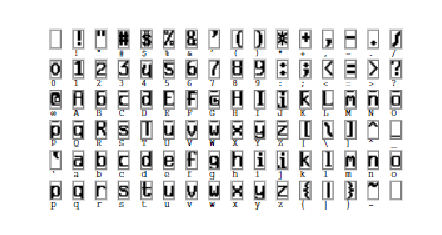
\includegraphics[width=80mm]{assets/3.eps}
  \caption{ASCII セットに対する出力}
  \label{fig:3}
\end{figure}

\par
出力に一般的な "1 of N" 符号ではなく, このような分散的な符号を用いるもう一つの理由として, クラスの数が数十といったオーダーより大きくなると, 非分散符号の動作が悪くなる傾向があるからである.
出力ユニット内の非分散符号は, ほとんどの時間非活性にならなければならない. これはシグモイドユニットではかなり難しい. さらにもう一つの理由は, 分類器は文字だけでなく文字以外の認識にも良く用いられるからである. 分散的な符号を持つ RBF は非典型パターンが外部に落ちやすいようによく囲われた入力の領域で活性化されるためこの目的に適している.
\par
RBF のパラメータベクトルは F6 のターゲットベクトルの役割を担う. これらのベクトルの成分は +1 あるいは -1 であり, F6 のシグモイドの範囲内であるため,シグモイドが飽和するのを防ぐことができる. 実際, +1 と -1 はシグモイドの曲率が最大となる点である.
シグモイドの飽和は, 損失関数の悪い条件付け, 収束が遅くなることにつながるため避けなければならない.

\subsection*{C. 損失関数}
上記のネットワークで使用できる最も簡潔な出力損失関数は, 最尤推定 (MLE) であり, 本研究では 最小平均二乗誤差 (MSE) と等価である.
学習サンプルの集合に対する基準は簡単である.
\begin{equation}
  E(W) = \frac{1}{P}\sum_{p=1}^{P}y_{D^p}(Z^p,W)
\end{equation}
ここで, $y_{D^p}$ は $D^p$ 番目の RBF ユニットの出力, すなわち入力パターン $Z^p$ の正しいクラスに対応するものである.
このコスト関数は, ほとんどの場合において適切であるが, 3つの重要な特性が抜けている. 
第 1 に, RBF のパラメータを適応させる場合, $E(W)$ は到底受け入れがたい解となる. この解では, すべての RBF のパラメータベクトルが等しく, F6 の状態が一定の場合にはそのパラメータベクトルに等しくなる.
この場合, ネットワークは入力を無視し, すべての RBF の出力は 0 に等しくなる破滅的な現象が起きる.
 2 つ目の問題は, クラス間で競合が起こらないことである. HMM における学習に使用される最大相互情報量に類似した MAP (maximun a posteriori) と呼ばれるより識別性能が高い学習基準を使用することで得ることができる.
 これは, 入力画像がクラスのうち 1 つに対応している, あるいは背景を表す 「ゴミ」 クラスラベルに対応しているとすると, 正しいクラス $D^p$ の事後確率を最大化 (あるいは正しいクラスの確率の対数を最小化) することに相当する.
 ペナルティの観点からは, MSE のように正しいクラスのペナルティを下げるだけでなく, 異なるクラスのペナルティを引き上げることができる.
 \begin{equation}
  E(W) = \frac{1}{P} \sum_{p=1}^P (y_{D^p}(Z^p,W) + \mathrm{log}(e^{-j} + \sum_{i}e^{-y_i(Z^p,W)}))
 \end{equation}
 第 2 項の負は競合の役割を果たす.
 第 2 項は, 第 1 項 に比べ小さい (あるいは等しい) ことが必要であるため, この損失関数は正である.
 定数 $j$ が正の値であり, すでにペネルティがかなり大きいクラスのペネルティをさらに引き上げるのを防ぐ.
 「ゴミ」クラスラベルの事後確率は, $\mathrm{log}(e^{-j} + \sum_{i}e^{-y_i(Z^p,W)})$ の割合である.
 この基準では RBF パラメータを学習するときに, RBF の中心を互いに離し先述した破壊的な影響を防ぐことができる.
 \par
 畳み込みネットワークの全層の重みに対する損失関数の勾配は逆伝搬法を使用して計算する.
 これを実装する簡単な方法は, 重みの共有がない従来の多層ネットワークであるかのようにネットワークの各接続に対して損失関数の偏導関数を計算し, その次に同じ重みパラメータを共有するすべての接続における偏導関数を追加し導関数を形成する.
 このような大規模なアーキテクチャはかなり効率的に学習することができるが, そのためにはさらにいくつかの技術を使用する必要がある. 

 \section{結果と他手法との比較}
 数字の認識タスクは, 形状認識手法を比較するためのベンチマークとして優れている. 
 本論文ではサイズ正則化された画像に対して直接的に動作する適応的な手法に焦点を当てている.

 \subsection*{A. データベース: 修正した NIST セット}

本論文でシステムの学習, 検証で用いるデータベースは NIST の Special Database 3 と Special Database 1 の手書き整数の 2 値画像である. SD-1 と SD-3 には手書き文字の書き手やデータのスクランブルといった差があり, 
学習データとテストデータの選択に実験結果が依存しないようにするために, NIST のデータセットを混合して新たなデータセット Modified NIST , MNIST を構築した.
実験では, 10000 個のテスト画像, 60000 個の学習データ画像を用いた. 
\par
元の 2 値画像は縦横比を保ったまま 20 × 20 ピクセルに収まるように標準化され, 標準化の過程でグレーレベルが含まれる.
データセットは以下の 3 つのバージョンを用いた.
1 つ目は, ピクセルの重心を計算し画像を平行移動することで 28 × 28 の領域の中心に配置した. これをレギュラーデータセットと呼ぶ. 
2 つ目は, 文字画像の画角を補正し 20 × 20 ピクセルの画像にトリミングする. 画角補正では, ピクセルの 2 次慣性モーメントを計算し, 主軸が垂直になるように線を水平方向にずらして画像を切り取る. 
画角補正済データセットと呼ぶ.
 初期の実験で用いられていた 3 つ目のデータセットは, 画像は 16 × 16 に縮小される. 図 \ref{fig:4} にテストデータからランダムに抽出した例を示す.
 \begin{figure}[t]
  \centering
  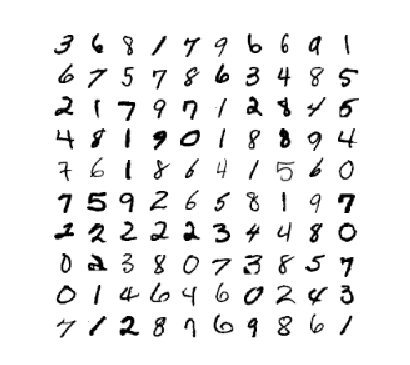
\includegraphics[width=80mm]{assets/4.eps}
  \caption{テストデータからランダムに抽出した例}
  \label{fig:4}
\end{figure}

\subsection*{B. 結果}
レギュラーデータセットを用いて, 複数バージョンの LeNet-5 を学習させた. 
各学習段階において学習データを 20 回反復した. 
学習率 $\eta$ は以下に示すように減少していく. 
最初の 2 回は 0.0005 , 次の 3 回は 0.0002, 次の 3 回は 0.0001, その次の 4 回は 0.00005, それ以降は 0.00001 とした. 
実験により過学習は起こらなかったが, 事前に計算した有効学習率の範囲内で学習率を比較的大きな値にしていたことが要因と考えられている.
\par
学習データの大きさの影響を 15000, 30000, 60000 として測定した. 図 \ref{fig:6} に学習時のエラーとテスト時のエラーを示す.

\begin{figure}[t]
  \centering
  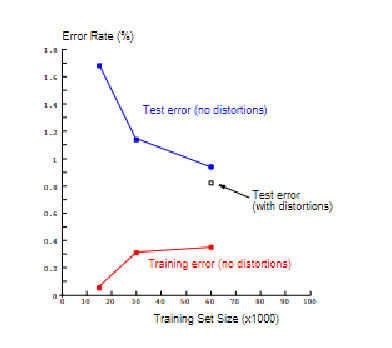
\includegraphics[width=80mm]{assets/6.eps}
  \caption{学習時のエラーとテスト時のエラー}
  \label{fig:6}
\end{figure}
LeNet-5 のような特殊なアーキテクチャでも, 学習データを増やせば精度が向上することがわかる.
\par
この仮説を検証するために, 学習用画像をランダムに歪ませることでデータ拡張を行い, 元の 60000 個の画像に加え, 540000 個の学習データを追加した. データ拡張は図 \ref{fig:7} に示すようにアフィン変換を適用した.
\begin{figure}[t]
  \centering
  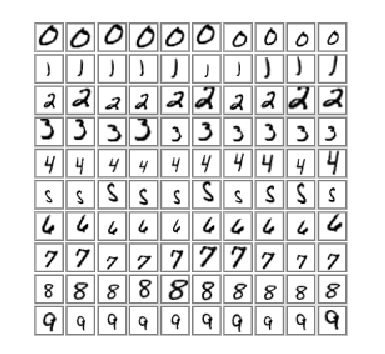
\includegraphics[width=80mm]{assets/7.eps}
  \caption{アフィン変換を施したデータ例}
  \label{fig:7}
\end{figure}
学習パラメータを変更せず, データ拡張を行った場合,テスト時のエラーは 0.95\% から 0.8\% に減少する. 
この 20 回の学習の繰り返しで, ネットワークは各サンプルを 2 回しか観測していない. 
図 \ref{fig:8} に誤分類されたテスト例を示している.
\begin{figure}[t]
  \centering
  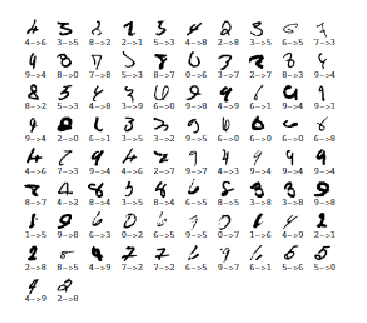
\includegraphics[width=80mm]{assets/8.eps}
  \caption{誤分類されたテストデータ例}
  \label{fig:8}
\end{figure}
例の中では, 人間から見ても曖昧なものもあれば, 容易に判別可能な例もある. 

\subsection*{C. 他の分類器との比較}
比較のために同じデータセットに対して様々な分類器を学習し, テストした.

\subsubsection*{C.1 線形分類器とペアワイズ分類器}
最も単純な分類器として考えられるのが, 各入力画素値は, 各出力ユニットの重み付き和に寄与し, 最大値を持つ出力ユニットが入力文字のクラスを示す線形分類器である.
レギュラーデータセットでは, テスト時のエラーは, 12 \% , ネットワークは 7850 個の自由パラメータを持つ. 画角補正済みデータセットでは, テスト時のエラーが 8.4 \% でネットワークは 4010 個の自由パラメータを持つ.
\par
線形分類器を単純に改良したものが, ペアワイズ分類器である. ペアワイズ分類器は各クラスを他のクラスから分離するために各ユニットを個別にラベル付けして学習したものであり, レギュラーデータセットではテスト時のエラーは 7.8 \% まで減少している.

\subsubsection*{C.2 ベースライン : 近傍分類器}
もう 1 つの単純な分類器として, 入力画像間のユークリッド距離を用いた K 近傍分類器がある.
この分類器は, 学習や設計が必要ではないという長所があるが, メモリ容量と認識にかかる時間が大きくなる欠点がある.
レギュラーデータセットにおいてはテスト時のエラーは 5.0 \% であった. 画角補正済みデータセットの場合, $k = 3$ の時にテスト時のエラーは 2.4 \% となった.
本研究で示す他のシステムはすべて画素を直接処理しているため, この分類器はベースラインとして適している.

\subsubsection*{C.3 主成分分析 (PCA) と 多項式分類器}
入力パターンを学習ベクトル集合の 40 個の主成分に投影するように前処理し, 主成分を計算した. 得られた 40 次元の特徴ベクトルは多項式分類器の入力として使用し, 結果としてこの分類器は前もって入力変数の組の積を計算しておく 821 個の入力を持つ線形分類器とみなすことができる.
レギュラーデータセットにおけるテスト時のエラーは 3.3 \% であった.

\subsubsection*{C.4 放射基底関数 (RBF) ネットワーク}
第 1 層が 28 × 28 入力の 1000 個のガウス型 RBF ユニットからなり, 第 2 層が単純な 1000 個の入力, 10 個の出力を持つ線形分類器となる RBF ネットワークを構築した,
RBF ユニットは 100 個ずつ 10 グループに分けられ, 適応的な k-means 法を用いて 10クラスのうちの 1 つずつすべての学習データについて RBF のユニットをグループごと学習した.
レギュラーデータセットにおいてテスト時のエラーは 3.6 \% であった.

\subsubsection*{C.5 1 つの隠れ層を持つ完全結合多層ニューラルネットワーク}

誤差逆伝搬法を用いて学習した 1 層の隠れ層を持つ多層ニューラルネットワークを構成し, 検証した.
レギュラーデータセットにおいてテスト時のエラーは 300 個の隠れユニットの場合は  4.7 \% , 1000 個の各ユニットの場合は 4.5 \% となった.
データ拡張を行った場合, 300 個の隠れユニットでは 3.6 \%, 1000 個の隠れユニットの場合は 3.8 \% とわずかな改善しか得られなかった.
画角補正済みデータセットにおいてテスト時のエラーは 300 個の隠れユニットで 1.6 \% に減少した.
このような多くの自由なパラメータを持つネットワークで低いテスト時の誤差が得られる原因として, 筆者たちは多層ニューラルネットワークにおける勾配降下法の挙動に「自己正則化」の効果があると推測しているが, まだ理論的な理解や実証的な根拠が必要であるとしている.

\subsubsection*{C.6 2 つの隠れ層を持つ完全結合多層ニューラルネットワーク}
28 × 28 - 300 - 100 - 10 ネットワークにおけるテスト時のエラーが 3.05 \% となり 1 つの隠れ層の場合と比べかなり良い結果を得られた. さらに 28 × 28 - 1000 - 150 - 10 の場合では 2.95 \% とわずかに改善されただけだった. データ拡張を行った場合, 28 × 28 - 300 - 100 - 10 ネットワークでは 2.50 \% , 28 × 28 - 1000 - 150 - 10 の場合では 2.45 \% と若干の改善が見られた.

\subsubsection*{C.8 小規模な畳み込みネットワーク : LeNet-1}
畳み込みネットワークは, 学習データを十分に学習できない小さなネットワークと過度にパラメータ化された大きいネットワークのジレンマを解決するための試みである.
入力画像は 16 × 16 ピクセルに縮小され, 28 × 28 の入力層の中央に配置された. LeNet-1 の評価には 100000 ステップの乗算加算が必要になるが, 畳み込み処理の性質上, 自由パラメータは約 2600 個に留まる.
LeNet-1 ではテスト時のエラーが 1.7 \% となり, パラメータが少ないネットワークで良い結果を残せていることは LeNet-1 のアーキテクチャがタスクに適していることを示している.

\subsubsection*{C.8 LeNet-4}
LeNet-1 と比較して大規模な学習データを最適に利用するために設計されたのが LeNet-4 である. LeNet-4 では, 4 つの特徴マップとそれに続く 8 つのサブサンプリングマップが第 1 層の各特徴マップに対として結合し, 次に 16 個の特徴マップと 16 個のサブサンプリングが続き, 17000 個の自由パラメータを持っている. テスト時のエラーは 1.1 \% であった.

\subsubsection*{C.9 ブーストした LeNet-4 }
複数の分類器を結合する「ブースティング」の手法がある. 1 つ目のネットワークは通常通り学習し, 2 つ目は 1 つ目のネットワークによって 1 番目のネットワークが正解したパターンと間違えたパターンが 50 \% づつ混在するようにフィルタリングされたパターンを学習する. 3 つ目のネットワークは 2 つのネットワークが間違えた新しいパターンで学習される. データ拡張し実験した結果, テスト時のエラーは 0.7 \% とどの分類器よりも優れていた. また, 計算コストも 1 つのネットワークの時に比べ約 1.75 倍であった.

\subsubsection*{C.10 タンジェント距離分類器 (TDC)}
TDC は入力画像の歪みや変換に敏感な距離関数を配置した最近傍法である. 画像を高次元の画素空間の点と考えると, 歪みは空間内の多様体を意味し, この多様体はタンジェント平面と呼ばれる平面で近似できる. 
文字画像の「近さ」は平面の距離で表される.
16 × 16 の画像を用いた学習では, テスト時のエラーは 1.1 \% となった.

\subsubsection*{C.11 サポートベクターマシン (SVM)}
SVM は高次元区間の複雑な局面を表現する際に非常に優れた方法である. 通常の SVM を用いた場合, レギュラーデータセットを用いた学習におけるテスト時のエラーは 1.4 \% であった.
通常のSVMを用いた時, Burges と Sch\"{o}lkopf によってレギュラーデータセットを用いてテスト時のエラーは1.4 \% という結果が得られた.その後, Sch\"{o}lkopf は V-SVM という SVM の改良版を用いて 0.8 \% という結果を得た. V-SVM は非常に計算コストが高いため, Burges は RS=SVM という手法を提案しレギュラーデータセットで 1.1 \% を記録した.

\subsection*{D. 考察}
図 \ref{fig:9} ~ \ref{fig:12} に分類器の性能の概要を示す. 
\begin{figure}[t]
  \centering
  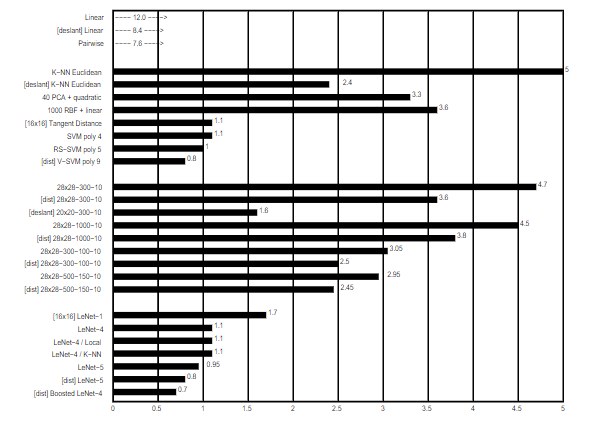
\includegraphics[width=80mm]{assets/9.png}
  \caption{10000 件のテストデータに対するエラー}
  \label{fig:9}
\end{figure}
図 \ref{fig:9} では 10000 件のテストデータに対するエラーを示しており, ブースティングを行った LeNet-4 が 0.7 \% と最も良い結果を残し, LeNet-5 の 0.8 \% がそれに続いた.
\par
図 \ref{fig:10} では, エラー 0.5 \% を達成するために棄却しなければならないデータ数を示している. 
\begin{figure}[t]
  \centering
  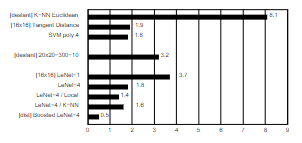
\includegraphics[width=80mm]{assets/10.png}
  \caption{エラー 0.5 \% を達成するために棄却しなければならないデータ数}
  \label{fig:10}
\end{figure}
多くのアプリケーションは テスト時のエラーよりもこの指標の方が重要である. ここでも ブースティングされた LeNet-4 が最も良い性能を残した. LeNet-4 の改良版はテスト時のエラーはほぼ同一だったものの, この指標では LeNet-4 より優れた結果を残した.
\par
図 \ref{fig:11} は各手法について 1 枚のサイズが標準化された画像を認識するために必要な積和演算の数を示したものである. 
\begin{figure}[t]
  \centering
  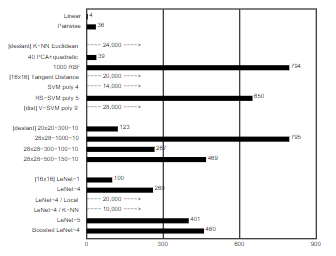
\includegraphics[width=80mm]{assets/11.png}
  \caption{標準化された画像を認識するために必要な積和演算の数}
  \label{fig:11}
\end{figure}
ニューラルネットワークはメモリベースの方式に比べてはるかに負担が少なく、畳み込みニューラルネットワークはその規則的な構造と重みのための必要なメモリが少ないことから積和演算の数も少ないことがわかる. 
\par
学習時間も計測した. k 最近傍法と TDC はほぼ学習時間は 0 であった.
一方で, 1 つの層からなるネットワーク, ペアワイズネットワーク, PCA + 2 次ネットワークは 1 時間未満で計算できる一方で, 多層ニューラルネットワークはより長い時間かかると予想されましたが, 実際には学習セットを 10 ~ 20 回繰り返すだけだった.
学習時間という指標は, 開発者にとっては重要だが, システムのユーザーにはほとんど意味がない.
\par
図 \ref{fig:12} には様々な分類器における記憶する必要のある変数の数で測定したメモリ要件を示している.
\begin{figure}[t]
  \centering
  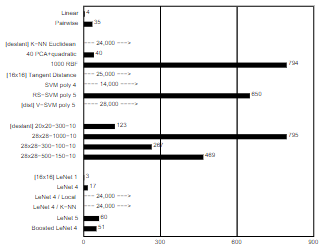
\includegraphics[width=80mm]{assets/12.png}
  \caption{様々な分類器におけるメモリ要件}
  \label{fig:12}
\end{figure}
ほとんどの手法は妥当な性能を得るために 1 変数当たり約 1 バイトしか必要としない. しかし, 最近傍法では  1 画素当たり 4 ビットのメモリで十分な性能を得ることができる.
当然, ニューラルネットワークはメモリベースの方法よりもはるかに少ないメモリしか必要としない.
\par
分類器の全体的な性能は, 精度, 実行時間, 必要なメモリなど多くの要因に依存する. 
1989 年の段階では, LeNet-5 のような複雑な分類器は数週間物学習が必要であり, 検討されていなかった.
LeNet-1 から様々な分類器が考案されたものの, 様々な学習機の性能の見積もりからより優れたニューラルネットワークアーキテクチャの期待が高まり, LeNet-4 や LeNet-5 が開発された.
\par
また, ブースティングによりメモリと計算機のコストを抑えながら精度を向上させることができることがわかった.
また, データ拡張により多くの元学習データが無くてもデータセットのサイズを増やすことができる.
\par
サポートベクターマシンは問題に対する事前知識を含んでいないため優れた制度を実現しているが, 畳み込みニューラルネットワークに匹敵する性能に達するにはメモリと計算機にかなりのコストがかかる. 
比較的新しい手法である縮小版 SVM はコストが畳み込みニューラルネットワークの 2 倍程度ではあるが, エラーの値は非常に近い. 
\par
多くの量のデータが利用可能な場合, 多くの手法で十分な精度を残すことができる. ニューラルネットワークを用いた手法はメモリベースの手法に比べて実行速度がかなり早く, コストも少ない.
ニューラルネットワークを用いた手法の優位性は学習データの規模が増えるほどより顕著になる.
\subsection*{E. 不変性とノイズ耐性}
畳み込みニューラルネットワークは実世界の文字認識システムにおけるヒューリスティックな分割によって生成されるようなサイズや位置が大きく変化する形状を認識するのに特に適している.
\par
上記の実験ではノイズ体制や歪み不変性の重要性は明らかではないが, 実際のアプリケーションにおいては全く異なる.
一般に文字は認識過程の前に分割する必要があるが通常は完璧にはいかず, 文字画像にノイズが残り前処理ができない画像となる.
そのため, 多くのシステムでは領域や単語のレベルで画像を正規化する. 本研究では, 上下のプロファイルを検出し, 一定の高さに正規化した. ただ, この方法では文字の大きさや縦方向の位置のばらつきが大きくなるため, ばらつきに強い認識器を用いることが望ましい. 実験では歪んだ文字, ノイズが含まれた文字に対してある程度の認識性能を得ており, このことから畳み込みニューラルネットワークが幾何学的な歪みに対する頑健性を持つ部分的な根拠が得られた.


\section{マルチモジュールシステムと GTN}
先述した逆伝搬法は, 勾配に基づく学習の単純な形態である.
しかし, (4) 式で示される勾配逆伝搬アルゴリズムは, 
線形層とシグモイド関数の交互の配置からなる単純な多層 FFN よりも一般的な状況を示していることは明らかである.
しかし, 大規模で複雑な学習システムは, 特化したモジュールから構築される必要がある. 
単純な例は 畳み込み層やサブサンプリング層, 完全連結層, RBF 層からなる LeNet-5 がある.
\par
マルチモジュールシステムは, 各モジュールが実装する機能とモジュール間の相互接続のグラフによって定義される. グラフはモジュールが更新されなければならない順序を示している.
最も単純なケースでは損失関数は, 望まれる出力を得られるような外部の入力を受け取る.

\subsection*{A. オブジェクト指向のアプローチ}
マルチモジュールシステムを実装する際, オブジェクト指向プログラミングは便利な方法である. 各モジュールはクラスのインスタンスであり, モジュールクラスは 「順伝搬」メソッドを持っている. 複雑なモジュールは単純なモジュールから新しいクラスを定義するで構築される.
このクラスの fprop メソッドは, 適切な中間状態変数や外部入出力を引数としてメンバモジュールの fprop メソッドをよびだすだけである.
ここでは, 有向非巡回グラフの場合に限定して述べる.
\par
マルチモジュールシステムにおける導関数の計算は簡単である. それぞれのモジュールのクラスにbprop と呼ばれる「逆伝搬」メソッドを定義できる. 
モジュールの bprop メソッドは fprop メソッドと同じ構成要素を持つ.

システムのすべての微分は, すべてのモジュールに対して bprop メソッドに対して順伝搬と逆順に呼び出すことで計算できる.
逆伝搬によりシステムのすべての状態変数とパラメータに関する損失関数 $E$ の偏導関数が効果的に計算される.
順伝搬と逆伝搬の間には興味深い二元性がある.
\par
導関数が逆伝搬により計算できることは直感的に理解しやすい. 理論的に正当化するには, ラグランジュ関数を用いる方法がある.
再帰的な接続を持つネットワークに拡張するために使用される.

\subsection*{B. 特殊モジュール}
ニューラルネットワークや他の標準的なパターン認識手法は, 勾配に基づく学習で学習したマルチモジュールシステムとして定式化できる.
一般的に使用されるモジュールには, 行列積やシグモイド関数などがあり, これらを組み合わせることで従来のニューラルネットワークを構築できる, その他も, 畳み込み層, サブサンプリング層, RBF 層などがある. 損失関数も 1 つのモジュールとして表現され, 一般的に使用されるモジュールは bprop メソッドを持つ. 一般的には, 関数 $F$ の bprop は, $F$ のヤコビアンとの乗算である.
 興味深いことに, ある種の微分不可能なモジュールはマルチモジュールシステムに悪影響を与えることなく挿入することが可能である.
 例として, マルチプレクサモジュール, min モジュールがあり, これらはある条件下においては微分可能であるため, 勾配に基づく学習アルゴリズムでも収束が保証されている.
\par
オブジェクト指向でのマルチモジュール実装は 2 次導関数のガウス-ニュートン近似を伝搬する bbprop メソッドを含むように簡単に拡張できる.
\par
マルチプレクサモジュールは, 一般的なシステムのアーキテクチャが入力データに応じて動的に変化する特殊なケースであり, 新しい入力パターンごとにアーキテクチャを動的に再構成するために使用することができる.

\subsection*{C. GTN}
マルチモジュールシステムは大規模な学習可能システムを構築するための非常に柔軟な道具である. しかし, 先述した章においてはパラメータと状態情報が組となって固定長のベクトルでモジュール間を通信していることが前提となっていた.
固定長のベクトルでデータを表現する場合には柔軟性に制約がかかり, このことは多くのアプリケーションで深刻な欠点となっている.
\par
より一般的には, 固定長のベクトルは, ベクトルや記号の系列に対する確率分布を符号化する必要があるタスクには柔軟性が欠ける. このような系列の分布は, 一般的には枝にベクトルが含まれる有向グラフで表現される. 
グラフの各パスは異なるベクトル列を表す. 各枝に関連するデータの要素を確率分布のパラメータとして解釈することで系列に対する分布を表現できる. また, グラフ内の各パスは入力の代替解釈を表す.
\par
本研究では大規模な手書きシステムを構築する際に, システムを 1 つ以上のグラフとして受け取り, 出力としてグラフを生成するモジュールのネットワークとみなすことで簡単かつ迅速に開発や設計できることを発見した.
このようなモジュールをグラフトランスファーと呼び, 出来上がったネットワークを GTN と呼ぶ.
\par
統計的な観点から見ると, 従来のネットワークにおける固定長の状態ベクトルは状態空間における分布の平均を表している.
状態が可変長である固定長のベクトルは, 固定長のベクトルの可変長の系列に対する確率分布の平均とみることができる.
また, GTN は状態はグラフとして表現され, 構造化されたベクトルの系列の確率分布の混合として見ることができる.
\par
勾配に基づく学習法は, GTN に一般化することができる.
グラフ変換器による勾配逆伝搬は, 出力グラフの数値情報に対して勾配を取り, さらに入力グラフとモジュール内部のパラメータの数値情報に対して勾配を計算する. 勾配計算の際の関数が微分可能であれば勾配に基づく学習法は適用可能である.
\par
また, 一般的にモジュールを組み合わせて用いる文書処理システムなどのシステム内のモジュール内部で実装されている関数がその内部パラメータや入力に対して微分可能であり, 大域的に学習可能なシステムとして使用できる.
\par
この 2 つのことを以下の章で示す. その際, あえて確率論への言及を避ける. 

\section{複数物体認識: ヒューリスティックオーバーセグメンテーション}
手書き文字認識における最も難しい問題の 1 つは, 分離した文字だけでなく, 文字列も認識することである. ほとんどの分類器は 1 度に 1 つの文字しか扱うことができないため文字列を個々の文字画像を分割する必要があるが, 自然に書かれた文字列を完全に正確に分割する画像解析技術を発案するのはほぼ不可能である.
\par
認識器を単語や分レベルで大域的な基準を最適化するように学習させることは, 個々の文字を認識するためだけでなく, 誤って分割された文字を拒否することもでき全体の誤差を最小にできるため好ましい.
\par
本章と次の章では, 単語や小切手などの文字列を読み取るための GTN の簡単な例について説明する. この方法ではセグメンテーションの結果を逐一人間の手で確認する作業を避けることができる.

\subsection*{A. 分割グラフ}
単語の分割と認識のための古典的な方法はヒューリスティック・オーバーセグメンテーションと呼ばれる手法である.
他の手法と比べて, 多数の異なる分割を考慮することでセグメンテーションに関する難しい決定を避けることができるという利点がある. この手法では, ヒューリスティックな画像処理技術を用いて単語, 文字列のカットの候補を見つけ次に認識器を使用して生成されたセグメンテーションを採点する.
カットの候補は必要以上の候補を生成する.
分割グラフは, 開始ノードと終了ノードを持つ有向非巡回グラフであり, 各ノードはカット候補に関連付けられており, 枝はカット間の画像に対応している. グラフを通る完全なパスは, 文字列を形成するためのセグメンテーションの断片を関連付ける方法に対応している. 

\subsection*{B. 認識変換器とビタビ変換器}
文字列を認識するための簡単な GTN を 図 \ref{fig:17} に示す.
\begin{figure}[t]
  \centering
  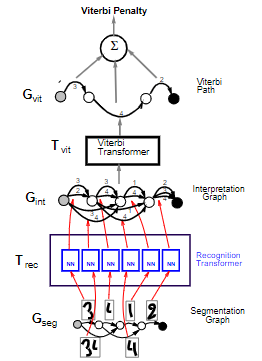
\includegraphics[width=80mm]{assets/17.png}
  \caption{文字列を認識するための簡単な GTN アーキテクチャ}
  \label{fig:17}
\end{figure}
 これは認識器 ${T_{rec}}$ , ${T_{vit}}$ の 2 つのグラフトランスフォーマーからから構成されている. 
認識変換器は, 解釈グラフ $G_{int}$ を生成することが目標であり, これは入力のすべての可能な分割すべての解釈を含むものである. $G_{int}$ の各パスは入力におけるうち 1 つの可能な解釈を示す. ビタビ変換器の役割は解釈グラフから最適な解釈を抽出することである. 
\par
認識変換器 $T_{rec}$ は, 分割グラフ $G_{seg}$ を入力として分割グラフの各枝に関連する画像に文字用の認識器を適用する.
解釈グラフ $G_{int}$ は, 各枝が同じノードからの枝と同じノードへの枝のセットに置き換えられることを除いて, $G_{seg}$ とほとんど同じ構造を持っている. 
$G_{int}$ の枝は $G_{seg}$ 内の枝に関連する画像の可能なクラスごとの数値を持つ.  
各枝にはクラスラベルと, 画像がクラスラベルへが示すクラスへ属するというペナルティが設けられている. 
分割機能によって分割候補に対するペナルティが計算されると, これらの制約は文字認識機能によって計算されたペナルティと組み合わせて解釈グラフの枝に対するペナルティが求められる. GTN の学習ではペナルティを調整し, 異なる性質のペナルティを組み合わせて利用する.
解釈グラフの各パスは, 入力された単語の解釈の可能性に対応する. ある分割に対応する特定の解釈のペナルティは解釈グラフの対応するパスに沿った枝のペナルティの合計で与えられる.
\par
ビタビ変換器は 1 つのパスをもつグラフ $G_{vit}$ を生成する. このパスは解釈グラフの累積ペナルティが最小のパスである. ビタビ変換器によって抽出されたグラフ $G_{vit}$ に沿った枝のラベルを読み取ることで認識結果を生成することができる. ビタビ変換器は, 動的計画法の原理を応用しグラフ内の最短経路を効率的に求めるビタビアルゴリズムから名付けられている. ソースノード $s_i$ と目的地ノード $d_i$ を持つ枝 $i$ に関連するペナルティを $c_i$ とする (2 つのノード間に複数の枝が存在する可能性に留意する). 解釈グラフでは, 枝もラベル $l_i$ を持つ. ビタビアルゴリズムは以下のように進行する. まず, 各ノード $n$ にはビタビペナルティの累積値 $v_n$ が設定され, これらの累積ペナルティは 0 で初期化される. 他のノードの累積ペナルティ $v_n$ はその親ノードの $v$ 値から上流の枝 $U_n = { \mathrm{arc} \: i \: \mathrm{with   \: destination} \: d_i = n}$を介して再帰的に計算される.
\begin{equation}
  v_n = \underset{i \in U_n}{min} (c_i + v_{s_i}).
\end{equation}   
さらに, 右辺を最小化する各ノード $n$ の $i$ の値を $m_n$ と示す. 終点ノードに到達したとき $v_{end}$ で, ペナルティの合計が最小となる経路を求める. この経路のペナルティををビタビペナルティと呼び, この枝とノードの系列をビタビパスと呼ぶ. ノード $n_1 ... n_T$ と枝 $i_1 ... i_T$ を持つビタビパスを得るには, これらのノードと枝を次のように辿る. 
終点ノード $n_T$ から始めて開始ノードに達するまで最小の枝: $i_t = m_{n_t + 1} and n_t = s_{i_t}$ を再帰的に辿る.
そしてビタビパスの枝からラベルの列を読み取ることができる.

\section{グラフ変換ネットワークのための大域的な学習}
本章では正しく分割された文字列における正しいクラスラベルには低いペナルティを, 違うクラスラベルには高いペナルティを, 正しく分割されなかった文字列に対してはすべてのクラスラベルについて高いペナルティを課すような文字列レベルでの認識システムの学習方法について説明する.
多くのアプリケーションでは各モジュールを別々に学習させるために多くの事前知識が用いられるが, これらを用いた個別学習は最適ではないことが知られている. 以下の章では GTN ベースの手書き文字認識器を文字列レベルで学習するための 3 つの異なる勾配に基づく学習法について説明する. 各手法はそれぞれビタビ学習, 判別ビタビ学習, フォワード学習である. 本研究では確率的な解釈に頼らず, 勾配に基づく学習における識別学習は誤差訂正学習の原理の単純な一例であることを示す. 
\par
HMM のようなグラフベースの系列認識システムのための学習方法は, システムがデータの確率的生成モデルに従い, 可能な入力系列の空間において正規化された尤度を提供する. 一般的な HMM 学習はこの正規化に依存しているため, ニューラルネットワークのような非生成的なモデルを組み込むと正規化を維持できない.
この場合には識別的学習法など他の手法を用いてニューラルネットワーク/ HMM 音声認識器を単語や文章レベルで適用する方法が提案されている. 
\par
他の大域的な学習可能な系列認識システムはグラフベースに頼らずに統計的モデリングの難しさを避けている. その最たる例が RNN であるが, 勾配に基づく学習を用いた RNN の学習は非常に困難であることが判明している. 以下に示す GTN 技術は音声認識のために開発された大域的な学習法を一般化したものである.
\subsection*{A. ビタビ学習}
認識時にはビタビアルゴリズムにより得られたペナルティの最も低い経路が正しいラベル列と関連していることが望ましい. よって最小化すべき損失関数は最も低いペナルティを持つ正しいラベル列の関連するパスの学習データセットの平均となる. 学習ではこの平均を最小化するような認識器のパラメータの集合を見つけることが目的となり, 損失関数の勾配は図 \ref{fig:19} に示す GTN アーキテクチャを介した逆伝搬法により計算される. 
\begin{figure}[t]
  \centering
  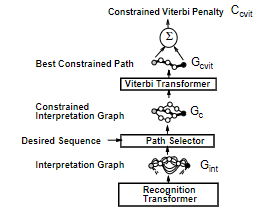
\includegraphics[width=80mm]{assets/19.png}
  \caption{ビタビ学習における GTN アーキテクチャ}
  \label{fig:19}
\end{figure}
図 \ref{fig:19} におけるパスセレクタと呼ばれるグラフ変換器は, 解釈グラフと最適なラベル列を入力として, 解釈グラフから相関のあるラベル列を含むパスを抽出する. 
その出力である制約付き解釈グラフ $G_c$ は正しいラベル列に対応するすべてのパスを含み, ビタビ変換器の入力となり 1 つのパスをもつ $G_{cvit}$ となる.
最後にパススコア変換器が $G_{cvit}$ を入力として累積ペナルティ $C_{cvit}$ を計算する. この GTN の出力は現在のパターンに対する損失関数である.
\begin{equation}
  E_{vit} = C_{cvit}
\end{equation}

このシステムでは希望する文字ラベルの並びのみ必要であり, 正しいセグメンテーションに関する知識は必要ない.
\par
ビタビ GTN のアーキテクチャで勾配を逆伝搬する過程において, 先攻するモジュールで勾配を計算したのちに勾配は GTN のすべてのモジュールを通して逆伝搬させる必要がある.
パススコア変換器においては, $G_{vit}$ 上の個々のペナルティに関する損失関数の偏導関数は損失関数がペナルティの和であることから 1 に等しいため単純である.
ビタビ変換器においては, $G_c$ の枝の制約に関する $E_{vit}$ の偏導関数は, $G_{cvit}$ に現れる枝については 1, そうでなければ 0 となる.
ビタビ変換器のような本質的に不連続な関数を逆伝搬させても良い理由としてはビタビ変換器が min 関数と加算器をまとめたものであるからである. 6 章で min 関数で勾配を逆伝搬しても悪影響がないことを述べた. 
パスセレクタにおける逆伝搬は, ビタビ変換器と同様である.
認識変換器においては, 順伝搬ではセグメンテーショングラフ内の各枝に 1 つずつインスタンスが生成され, $G_{int}$ の各枝のペナルティはインスタンスの出力により生成され, インスタンスは各出力に対する勾配を持つ. 逆伝搬では各インスタンスを通して勾配を逆伝搬することができる. 各インスタンスにおいてパラメータに関する損失関数の偏微分のベクトルを得る. すべての認識器インスタンスは同じパラメータベクトルを共有するため, 認識器の完全な勾配は単純に各インスタンスによって生成される勾配ベクトルの和となる. 
\par
このアーキテクチャは一見シンプルに見えるが, 致命的な欠陥がある. 認識器がシグモイド出力ユニットを持つ単純なニューラルネットワークである時, 損失関数の最小値は, 出力をすべての成分について小さな値を持つ一定のベクトルに設定することで達成され, 入力は無視される.
認識器の出力層が固定されたパラメータを持つ RBF ユニットを含む場合, 厳密には上記のような完全な崩壊は起こらないがより緩やかな崩壊は完全に防ぐことができない. また RBF のパラメータが適用可能であるなら, ニューラルネットワークが緩やかな崩壊を起こすベクトルを生成することを学習してしまい別種類の崩壊が起こってしまう. 
このような崩壊はニューラルネットワークのような学習可能なモジュールが RBF に入力した場合のみ発生する.
また, ビタビ学習では制約値が低い競合回答が考慮されないため, 解答の性能として信頼性が低くなってしまう問題もある.

\subsection*{B. 判別型ビタビ学習}
危険なほど低い制約値をもつようなおそらく間違えているパスのペナルティを上げるといったように学習基準を修正することにより, 上記の崩壊問題を回避すると同時により信頼性の高い評価値を生成できる. このような基準は, 識別的と呼ばれ個々のクラスを独立にモデル化するのではなく, クラス間に適切な分離面を構築しようとするものである. 識別基準の一例として, 所望の出力を満たすグラフにおけるビタビパスのペナルティと, 解釈グラフにおけるビタビパスとのペナルティの差, すなわち最良の正しいパスのペナルティと, 最良の正しいかどうか不明なパスのペナルティの差が挙げられる. 図 \ref{fig:20} に対応する GTN アーキテクチャを示す.
\begin{figure}[t]
  \centering
  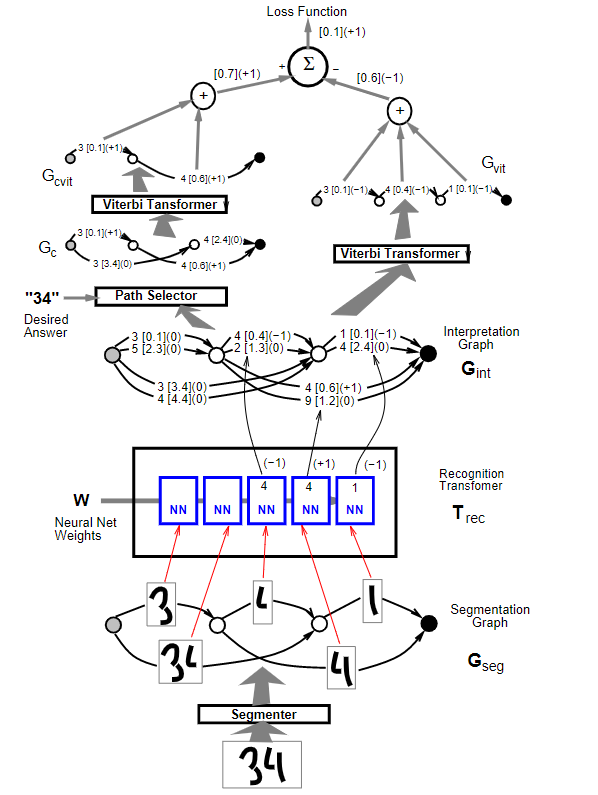
\includegraphics[width=80mm]{assets/20.png}
  \caption{判別型ビタビ学習に対応する GTN アーキテクチャ}
  \label{fig:20}
\end{figure} 
非識別学習では図 \ref{fig:20} の左半分で計算された所望の出力と図 \ref{fig:20} の右半分で計算された実際の出力の差を最小化する.
\par
判別ビタビ損失関数を $E_{dvit}$ とし, 所望の出力を得るグラフのビタビパスのペナルティを $C_{cvit}$, 解釈グラフのビタビパスのペナルティを $C_{vit}$ と呼ぶことにする.
\begin{equation}
  E_{dvit} = C_{cvit} - C_{vit}
\end{equation} 
なお, $E_{dvit}$ は常に正であり理想的なケースでは 0 となる. 
\par
判別ビタビ GTN における勾配の逆伝搬は, 図 \ref{fig:20} の右側はビタビ学習 GTN と同様で, $G_{int}$ の枝状の勾配では図 \ref{fig:20} の左側から負の寄与を受ける. $G_{int}$ の枝で $G_{vit}$ にも $G_{cvit}$ にも現れない枝は勾配は 0 となる. また, $G_{vit}$ と $G_{cvit}$ 両方に現れる枝の勾配も 0 となる. 言い換えれば, 枝が正解のパスに含まれているなら勾配は 0 となる. $G_{cvit}$ に存在して $G_{vit}$ に存在しない枝の勾配は +1 となりこの枝は $G_{vit}$ に含まれるようにより低いペナルティを持つべきであるといえる.
その反対の場合, 枝の勾配は -1 となりこの枝は望まれる解に含まれないためより高いペナルティを持つべきといえる. 
\par
判別ビタビ学習ではビタビ学習のような目立った欠陥はないが, 残存する問題としてはクラス間にはっきりとしたマージンを築いていないことである. そのため間違ったパスのペナルティが望ましいパスのペナルティに近づいたときに押し上げることができれば望ましいといえる.
\subsection*{C. フォワードスコアリング, フォワード学習}
ビタビパスの制約は認識という目的に適しているが, 状況の部分的な判断材料にしかなりえない. 同じ分割に対応する複数の最小ペナルティパスが同じラベル系列を生成する場合, 1 つのパスのみがその解釈を生成する場合よりも, そのラベル列が正しいという証拠になるため全体のペナルティはより小さくなるといえる.
確率論的な枠組みでは, 解釈の事後確率はその解釈を生み出すパスの事後確率の総和であるべきで, 解釈に対応するペナルティは個々のパスのペナルティの負の指数和の負の対数であるべきである. このような確率論的な枠組みでは, 全体のペナルティは個々のパスのすべてのパスより小さくなる. 
\par
解釈が与えられた時に上記の計算を効率的に計算するために フォワードアルゴリズムが知られている. また, これにより計算される特定の解釈に対するペナルティをフォワードペナルティと呼ぶ.
特定のラベル列と一致するパスだけを含む解釈グラフの部分グラフをペナルティグラフと呼び, ある解釈が与えられた時対応するペナルティグラフ上でフォワードアルゴリズムを実行すると解釈に対応したフォワードペナルティを得る. フォワードアルゴリズムはビタビアルゴリズムと非常によく似ているが, 累積ペナルティを組み合わせる際の演算が min 演算ではなく以下に示すいわゆる logadd 演算であることが違いである. 

\begin{equation}
  f_n = \mathrm{logadd}_{i \in U_n}(c_i + f_{s_i})
\end{equation}
ここで, $f_{\mathrm{start}} = 0$, $U_n$ はノード $n$ の常駐の枝の集合, $c_i$ は枝 $i$ のペナルティであり,
\begin{equation}
  \mathrm{logadd}(x_1, x_2,...,x_n) = -\mathrm{log}(\sum_{i=1}^{n}e^{-x_i})
\end{equation}
である.
枝に加算されるペナルティではなく, 乗法的なスコア : score = exp(- penalty) を考えると, ビタビアルゴリズムでは累積スコアが最大の経路を選択し, スコアはその経路に沿って乗算される. 一方, フォワードアルゴリズムにおけるスコアは開始ノードから終了ノードまでの各経路に関連する累積スコアの合計である. フォワードペナルティは常に他のパスの累積ペナルティよりも低い. ただし, ペナルティが他の経路に比べてかなり低い 「支配的な」経路が存在する場合, そのペナルティはフォワードペナルティとほぼ等しくなる. 
\par
フォワードペナルティを用いることで, ビタビアルゴリズムと比較して最も低いペナルティを持つ方法だけでなく, 答えを生成するすべての異なる方法を考慮することができ分割に曖昧さを含む場合に特に有効である. 
\par
フォワード学習 GTN は先述したビタビ学習 GTN におけるビタビ変換器を, 解釈グラフを入力としてそのグラフのフォワードペナルティを出力とするフォワードスコア計算機に置き換え, 最良の経路 1 つではなく正解を含むすべてのパスのペナルティを低くするように変更した GTN といえる.
\par
フォワードスコア計算機における逆伝搬はビタビ変換器とは異なる. グラフの各ノード $n$ で計算されたフォワード制約値 $f_n$ に対する微分はグラフ $G_C$ を介した逆伝搬により計算される.
\begin{equation}
  \frac{\partial E}{\partial f_n} = e^{-f_n} \sum_{i \in D_n}\frac{\partial E}{\partial f_{d_i}} e^{f_{d_i} - c_i}
\end{equation}
ここで, $D_n$ はノード $n$ の下流の枝の集合である. 上記の導関数から枝の制約に関する導関数が得られる. 
\begin{equation}
  \frac{\partial E}{\partial c_i} = \frac{\partial E}{\partial f_{d_i}} e^{- c_i - f_{s_i} + f_{d_i} }
\end{equation}
$G_C$ のすべての枝が損失関数に影響を与え, 低い制約値を持つパスに属する枝ほど大きな影響力を持つ. 

\subsection*{D. 判別型フォワード学習}
フォワードペナルティに含まれる情報は識別的フォワード基準と呼ぶべき別の識別的学習基準に利用することができ, この基準は正しい解釈に関連する経路を選択する事後確率を最大化することに相当する. 正しい解釈を持つパスに関連する事後確率がほぼ 1 になることは, 制限付きグラフのフォワード制約値が完全な解釈グラフのフォワード制約値と等価になることを意味するためこの状況になることが好ましい.
対応する GTN アーキテクチャの概要を図 \ref{fig:21} に示す.
\begin{figure}[t]
  \centering
  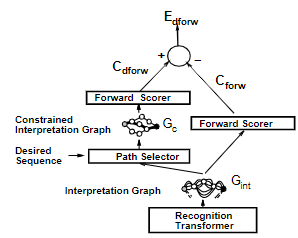
\includegraphics[width=80mm]{assets/21.png}
  \caption{判別型フォワード学習における GTN アーキテクチャ}
  \label{fig:21}
\end{figure}
\par 
差分を $E_{dforw}$, 制限付きグラフ, 完全な解釈グラフのフォワードペナルティをそれぞれ $C_{cforw}$, $C_{forw}$ とする. 
\begin{equation}
  E_{\mathrm{dforw}} = C_{\mathrm{cforw}} - C_{\mathrm{forw}}
\end{equation}
$E_{dforw}$ は, 解釈グラフと制限付きグラフの包含関係から常に正である. 先述した理想的な場合には $E_{dforw} = 0$ となる.
\par
判別可能なフォワード GTN で導関数を逆伝搬すると, ビタビの場合よりも勾配が均等に分散される. 導関数は図 \ref{fig:21} の左半分から解釈グラフまで逆伝搬され, また負となり右半分へも逆伝搬され左半分の結果に加えられる. 正しいパスの 1 部となる枝は正の導関数を持ち, この導関数は不正確なパスがすべての正しいパスよりも低いペナルティを持つ場合に非常に大きくなる. 同様に, 低いペナルティを持つ不正確なパスの 1 部となる枝に関する導関数は大きな負の導関数を持つ. 一方で, 正しい解釈に関連するパスのペナルティが他のすべてのパスよりはるかに小さい場合, 損失関数の値は 0 にほとんど近くなり勾配はほとんど逆伝搬されない. よって学習は分類誤りをもたらすデータに集中し, さらに誤りを引き起こす画像の断片に集中する.
一般的には学習機が離散的な代替解釈を選択ならなければならない状況で同じ考えを用いることができるエレガントな手法である.
\subsection*{E. 識別学習における備考}
先述した議論において大域的な学習基準に確率的な解釈を与えたが, グラフの枝の制約値については確率的な解釈を与えなかった. これには理由があり, 例えば和が 1 にならなければいけない, あるいは入力領域上で積分して 1 にならなければいけないなどの制約が異なるクラスラベルに関連する場合に問題が発生するためである.\par
クラスラベルの和が 1 にならなければいけないケース (クラスの正規化) においては, 画像の 1 部が有効なクラスに対応しない場合に分割候補が間違っている可能性があるとして局所的にすべてのクラスに対応しないために重要な情報を排除する可能性がある. Baum-Welsh アルゴリズムと Expectation-Maximization 法の組み合わせでは個々の変数の確率的な解釈が重要である. しかし, これらの方法は識別的な学習基準に適しておらず, 勾配に基づく学習においても非効率になりうる.\par
また, 入力領域上で積分して 1 にならなければいけないケース (入力の生成モデルを使用) について, 生成モデルは各クラスについての独立した密度モデルを構築しそのモデルに基づいて独立した分類の決定をすることで間接的な境界を構築する. これは分類判定面を学習するという学習における最終目標とは直接関係していないため識別的なアプローチではない. 
\par
分類のための内部変数が確率論的な解釈を持っていなくても, システム全体はクラスの事後確率を生成していると見なすことができる. 例えば先述した図 \ref{fig:21} においてあるラベル系列が「望ましい列」として与えられるとすると仮定すると, $-E_{dforw}$ の指数はラベル列の事後確率の推定と相互的に予測可能である. 
誤分類の数の近似値を直接最小化するといったアプローチがあるが, 本研究では最適化の際の数値的な問題が小さくなる, 分類モデルに適切と思うパラメータを自由に選択することができるという利点で判別可能なフォワード損失関数を用いている.

\section{複数物体認識 : 空間変位ニューラルネットワーク}
文字列の画像に対してヒューリスティックな分割を用いるかわりに, 正規化された画像のすべての可能な位置で認識器を適用する方法がある. 
しかし, この方法は大きく 3 つの問題がある. 1 つ目は計算コストが非常に大きいこと. 2 つ目は認識器が認識すべき文字の中心にある時, 認識器は近傍に他の文字があったとしても必ず正確に文字を認識しなければならないということ. 3 つ目は認識器がずれやサイズの変動に対してけんろうであることである. これらの問題は入力領域上で CNN を複製すればエレガントに回避できる. 第 3 章で述べたように CNN は入力画像のずれや大きさの変化, ノイズに対して非常に頑健である. このことで 2 つ目, 3 つ目の問題を回避できる. また, CNN は Space Displacement Neural Network (SDNN) と呼ばれる複製した CNN を用いる手法で大きな入力領域上で計算量を大幅に削減することができる. 入力領域上の CNN のインスタンスと近い場所にある CNN を考えると, CNN の性質上同じ出力を持つため, 共有されていない「スライス」だけが再計算される. その結果特徴マップが水平方向に大きくなっていることを除いて元のネットワークと同じ構造を持つ. 
SDNN は信頼できる分割方法が存在しない筆記体の認識タスクにおいて非常に魅力的である. SDNN のアイデアは非常に古く先述したように認識器への要求性能が高いため最近までは注目されていなかった. 
\subsection*{A. GTN による SDNN の出力の解釈}
SDNN の出力は入力の対応の位置で特定のクラスラベルを持つ文字を見つける尤度や制約値, あるいはスコアを符号化したベクトルの系列である.
このベクトル列から最適なラベル列を抽出するために後処理が必要となる.
SDNN においては個々の文字が複数の隣接する認識器のインスタンスに発見される, あるいは文字の一部しか見ていない認識器インスタンスによって誤って検出されることが高頻度で起こる.
出力列からこういった文字を防ぐには 図 \ref{fig:24} のような 2 つの入力グラフを持つグラフ変換器を用いる.
\begin{figure}[t]
  \centering
  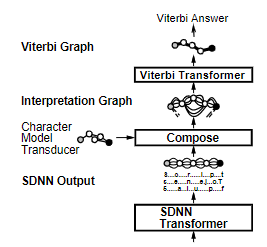
\includegraphics[width=80mm]{assets/24.png}
  \caption{SDNN を基とする GTN アーキテクチャ}
  \label{fig:24}
\end{figure}
SDNN が生じるベクトル列は隣接ノード間で複数の枝を持つグラフに変換される.
各枝はクラスのラベルと SDNN が生成するペナルティが含まれる. これを SDNN 出力グラフと呼ぶ.
2 番目の入力グラフは文字モデル変換器と呼ばれクラスラベルの文字列と認識された文字列の対応する出力文字列間の関係を符号化する. この変換器は重み付き記号系列を他の重み付き記号系列に変換する. 図 \ref{fig:24} のグラフ変換器は SDNN 出力グラフのすべてのパスに対応する系列を文字モデル変換器とマッチングさせることで SDNN 出力グラフと文字モデル変換器を合成変換器に通して解釈グラフを生成する. 解釈グラフには対応する出力ラベル列のパスが含まれる.
\subsection*{B. SDNN を用いた実験}
本章で示す実験では LeNet-5 が分割なしに複数の文字を認識するように複製されることを目標に学習を進めた. データセットは先述した修正データセットにおいて画像処理を施したものを用いた.
図 \ref{fig:26} は LeNet-5 SDNN が複数の文字認識に成功した例である. 
\begin{figure}[t]
  \centering
  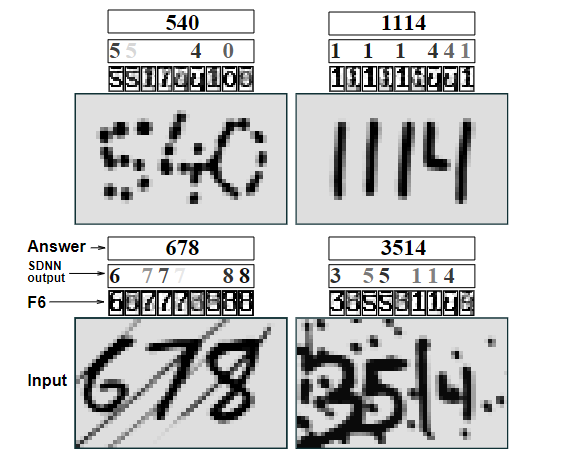
\includegraphics[width=80mm]{assets/26.png}
  \caption{ LeNet-5 SDNN が複数の文字認識に成功した例}
  \label{fig:26}
\end{figure}
LeNet-5 SDNN は顕著な不変性と耐ノイズ性があることが示された. 
また, 文字が密接に絡み合っている場合でも文字を区別することができている. さらに図 \ref{fig:26} の左上の例のように文字を形成する切断されたインクの断片から文字のグループ化に成功している.
図 \ref{fig:26} の右上の例では連続する 1 を幾何学的な外部情報なしで認識しており, 最後の 4 についても文字モデル変換器によって 1 と誤識別された結果が取り除かれて正しく認識されている. 
SDNN はこのような頑健性だけでなく, その「簡単さ」のため並列ハードウェアに実装することができることも利点として挙げられる.

\subsection*{C. SDNN の大域的な学習}
上記の実験では, 文字列画像は人工的に生成された画像であるため重要な文字の位置とラベルがあらかじめわかっていることになる. 実用上は文字列に対するラベルの正確な系列は入手可能であるが, 入力画像中の対応する各文字の正確な位置は不明となる. SDNN の大域的な学習では, 6 章で述べたようなアーキテクチャに配置された図 \ref{fig:27} のようなグラフ変換器を介して勾配を逆伝搬することによって可能となる. 
\begin{figure}[t]
  \centering
  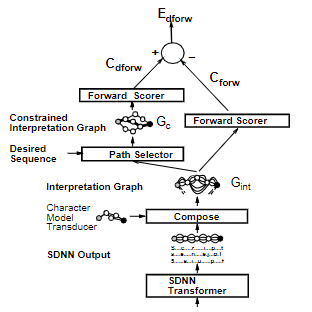
\includegraphics[width=80mm]{assets/27.png}
  \caption{SDNN の大域的な学習における GTN アーキテクチャ}
  \label{fig:27}
\end{figure}
これは SDNN の出力を隠れマルコフモデルでモデル化するのとほとんど同じである. 大域的に学習された可変サイズの TDNN/HMM ハイブリッドは様々な分野に用いられている. 
図 \ref{fig:27} は SDNN/HMM ハイブリッドを識別的フォワード基準で学習するためのグラフ変換器アーキテクチャである. 
図 \ref{fig:27} の右側では SDNN 出力系列と文字モデル変換器の合成によりすべての可能な解釈を示す解釈グラフを得る. 左側はさらに望まれるラベル系列を持つパスのみを含む文法と合成する. 損失関数は左半分から得られたフォワードスコアと右半分から得られたフォワードスコアの差である. 
合成変換器を逆伝搬するには, SDNN 出力グラフのどの枝が解釈グラフのどの枝を発生させたか記録する必要がある. SDNN 出力グラフ内の枝に関する導関数は, その枝を始点とする解釈グラフのすべての枝に関する導関数の和に等しい. 同様に文字モデル認識器の制約値についても導関数を計算できる. 先述したようにネットワークの出力 RBF が適応的である場合には破綻が起こりえるため識別的基準を用いなければならない. 
SDNN は非常に有望な技術であるが, ヒューリスティックな分割よりも良い結果を残せていない. これは今後の課題である.

\subsection*{D. SDNN による物体検出と注目}
SDNN と大規模な入力領域と親和性の良さが相まって大規模画像における「総当たり的な」物体の発見と検出に利用できることが示唆されている.
1 つの CNN を学習させ背景の画像から目的の物体の画像の画像を区別するといったことがアイデアとして考えられる. 
ネットワークは入力画像を分析するために画像全体を覆うように複製され結果的に 2 次元空間変異ニューラルネットワークが形成される, SDNN の出力は 2 次元平面となり活性化されたユニットがその中にあれば, 受信領域に注目する物体が存在することを意味する. 画像内の対象物体の大きさは未知であるため画像を複数の解像度でネットワークに通し, 複数の解像度の結果を結合することで結果を示すことが可能である. このアイデアは顔の位置検出などに応用されている.\par
画像中の顔検出の場合を考えると, 顔を含む画像を収集し, ラプラシアンフィルタで照明の変動と低い空間周波数の照明勾配が除去される. 次に, 手動でサンプルを抽出し顔の部分をサイズ正規化する. 背景画像の大きさはランダムに選択され, これらのサンプルに対して CNN が学習し, 顔部分画像と非顔部分画像を識別する.\par
画像を解析する際, ラプラシアンフィルタを通してから 2 のべき乗の解像度でサブサンプリングしネットワークは複数の解像度の画像に対してそれぞれ複製される. 結果の結合は単純な投票処理が用いられる. 
\par
前の章の大域的な学習手法の 2 次元版を用いることで学習サンプルを作成する際に顔の位置を手動で特定する必要性を削減できる.
\par
他の研究では顔検出に NN や SVM のようなクラス分類器を用いて大きな成功を収めている. これらは複数のスケールでネットワークに画像を通すというアイデアを含めて上記手法と非常に似ている. しかし CNN を用いていないため CNN の高速化が生かせず, 高速化のために他の手法を併用している. それに加えて これらのクラス分類器は CNN に比べて頑健性が低いため分類器に通す画像を増やさなければならない. 

\section{GTN と変換器}
この章では GTN を 一般化変換の枠組みで再解釈し強力なグラフ合成アルゴリズムを提案する

\subsection*{A. 先行研究}
音声認識においては, グラフベースの統計モデルと音響認識モジュールを統合する勾配型学習が用いられている.
しかし, 多層グラフを用いた学習可能なシステムにおいてのシステマチックなアプローチは提案されていない. 
グラフを他のグラフに変換するアイデアは CS の分野で大きな注目を集めており, 手書き文字のための提案もなされている. この研究では変換器かとグラフを組み合わせることによる代数的な側面について述べているが, 変換器から大域的に学習可能なシステムを構築するという点にはほとんど触れられていない. 
本研究ではグラフを操作するシステムの自動的な学習のためのアプローチを提案する.

\subsection*{B. 標準的な変換器}

有限状態変換器の枠組みでは, グラフの枝に離散的な記号がつけられている. 変換器グラフは入力記号と出力記号の 2 つを持ち, アクセプタグラフは各枝に 1 つの記号を持つ. この枠組みでは合成操作はアクセプタグラフと変換器グラフを入力として新たなアクセプタグラフを構築する.
合成操作はアクセプタグラフと変換器グラフを構築し, 出力アクセプタグラフの各パス $S_{out}$ は, 入力アクセプタグラフの 1 つのパス $S_{in}$ と変換器グラフの入出力系列のペアと 1 つのパスに対応する. 
出力アクセプタグラフの枝状の重みは入力アクセプタグラフと変換器グラフのマッチングからの重みを加算して得られる. 
以降, このグラフ合成操作を変換操作と呼ぶ. 
変換の例を図 \ref{fig:28} に示す. 
\begin{figure}[t]
  \centering
  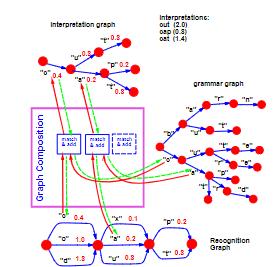
\includegraphics[width=80mm]{assets/28.png}
  \caption{グラフ合成操作の例}
  \label{fig:28}
\end{figure}
変換器の枝状の出力記号と入力記号は常に同一であり, このタイプの変換器グラフは文法グラフと呼ぶ.
2 つのトークンが入力アクセプタグラフと変換器グラフの開始ノードにそれぞれいると仮定すると, 両方のトークンがグラフの終端ノードに到達したとき許容可能な軌跡を持つ. 
この軌跡はアクセプタグラフと変換器グラフの両方に準拠した入力記号の並びを示している. 次に, 軌跡の沿って対応する出力記号列を集めることができる.
\par
この変換操作は非常に効率的であるが, 枝にラベル付けされている null と非 null 記号のすべての組み合わせの処理が複雑である. 重みが的確に正規化され確率として解釈される場合, アクセプタグラフはグラフ内のすべての可能なパスに関連するラベル系列集合によって定義される言語上の確率分布を示す.
変換操作の応用として単語などの文字列を認識する際に言語的制約を取り入れることが挙げられる. この例では各分割候補に関してニューラルネットワーク認識を適用してアクセプタグラフを作成する. このアクセプタグラフは文法の変換器グラフと一緒に構成される. この文法変換器には有効な記号列のパスが含まれ, 枝には同一の入力記号と出力記号が含まれる. 

\subsection*{C. 一般化した変換}
各枝に関連するデータが有限個の値しかとらない場合, 入力グラフを合成し変換器を使用することは妥当であるが, 画像認識といった場合グラフの枝のデータ構造はベクトルや画像, その他の高次元のオブジェクトとなる. そのためこれを解決する新しい合成操作を紹介する. 
\par
このような複雑なグラフを構成するには, さらに情報を追加する必要がある. 
\begin{itemize}
  \item 各入力のグラフから 1 組の枝を調べる時, 入力グラフの枝に付加された情報に基づいて出力グラフに対応する枝とノードを作るかどうかの基準が必要である. これにより枝, 複数の枝, あるいは複数のノードと枝からなるサブグラフ全体を構築することを決めることができる.
  \item この基準を満たした場合, 出力グラフに対応する枝とノードを作成し, 新たに作成された枝に付与する情報を計算する必要がある.
\end{itemize}
これらの機能はコンポジション変換と呼ばれるオブジェクトにカプセル化されている. 
このインスタンスは 3 つのメソッドを実装している.
\begin{itemize}
  \item check(arc1, arc2)
  \par
  arc1 と arc2 が持つデータ構造を比較して対応する arc を出力グラフに作成すべきするかどうかを返す.
  \item fprop(ngraph, upnode, downnode, arc1, arc2)
  \par
  check が True を返すと呼び出される. 出力グラフ ngraph のノード upnode と downnode の間に新しい枝とノードを作成し, これらの新しく作成した枝に付属する情報を計算する.
  \item bprop(ngraph, upnode, downnode, arc1, arc2)
  \par
  arc1 と arc2 のデータ構造, また同じ引数で fprop を呼び出した際に使用したパラメータに関して upnode と downnode の出力部分グラフから勾配を伝搬させるために学習中に呼び出される. 
  これは fprop の計算に用いる関数が微分可能であることを前提としている.
\end{itemize}
check 関数で動的なアークテクチャを構築し, fprop 関数でそのアーキテクチャを通して枝に付加された数値情報を計算する. bprop 関数ではアーキテクチャを逆伝搬して枝に付与された情報に対する損失関数の偏導関数を計算する. 
図 \ref{fig:29} は一般化されたグラフ合成アルゴリズムを簡略化したものである. 
\begin{figure}[t]
  \centering
  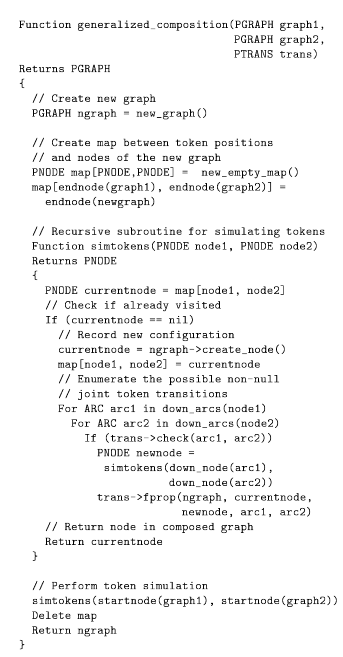
\includegraphics[width=80mm]{assets/29.png}
  \caption{簡略化したグラフ合成アルゴリズムの疑似コード}
  \label{fig:29}
\end{figure}
このアルゴリズムは Null 遷移は扱われず, 両方のトークンが同時にそのグラフの端点に到達する. null 遷移を管理するには各トークンの null 繊維の可能性を再帰的にシミュレーションし, 最終的に fprop 関数を呼び出せばよい. 許容可能な軌跡を特定する最も安全な方法は終端ノード上の両方のトークンに到達可能なトークンの構成を特定するの副次的なパスを実行することであり, これは逆方向の軌跡を列挙することで容易に達成できる. 
変換器を用いたグラフ合成は, 一般化された変換として簡単かつ効率的に実装される. check 関数は 2 つの枝状の入力記号を比較し, fprop 関数は変換器の枝状の出力記号を記号とする枝を生成する. 
グラフのペア間の合成は, 手書き文字認識装置に言語的制約を組み込む際に特に有効である. 
本論文の残りの部分では, 複数のグラフの変換に基づくグラフ変換器を示す. これまでに紹介されてきた分割器や認識器といったグラフ変換器の多くは一般化された変換の観点から定式化できる. 
この場合, 変換の入力は 1 つのグラフとなり, (check, fprop) のペアそのものが手続き的に変換器を定義しているとみなすことができる. 実際には生成されるグラフは手続き的に表現され, 認識時に探索アルゴリズムが訪れるノードだけをインスタンス化する. このことでビームサーチに代表される刈込アルゴリズムの利点がグラフ変換ネットワーク全体に伝搬される.

\subsection*{D. グラフ構造に関する注意点}
bprop 関数は一般的なグラフ変換器における逆伝搬アルゴリズムの基礎となるものである. check 関数が関係を確立すべきと判断すると, fprop 関関数が数値の計算を実行し, ネットワークの構造が確立される. 
fprop は微分可能であると仮定しているため勾配はネットワークのアーキテクチャに沿って逆伝搬することができ, ほとんどのパラメータがシステムのグラフの枝に格納されたスコアに影響を及ぼす. グラフに枝が現れるか否かを決定できる閾値パラメータもあり, ここではそのパラメータについてのみ考察する. 
これまで述べてきたようなシステムでは, グラフ変換器によって生成されるグラフの構造に関してはグラフ変換器の性質によって決まるが, パラメータの値や入力に依存することもあり得る.

\subsection*{E. GTN と隠れマルコフモデル}
GTN は HMM の一般化及び拡張とみなすことができる. GTN は複数のモジュールをフレームワークにより組み合わせることで HMM を拡張する.
\par
HMM を時間的に展開すると, 解釈グラフと非常に似たグラフが得られる. これはモデル内の各時間ステップ $t$ と状態 $i$ に関連するノード $n(t,i)$ を持つ.  $n(t-1, i)$ から $n(t, i)$ への枝のペナルティ $c_i$ は時間空間において位置 $t$ の観測データ $o_t$ が放出されて状態 $j$ から $i$ に至る負の対数確率に相当する. 確率論的に解釈するとフォワードペナルティは観測データ列の尤度の負の対数である. 
\par
6 章では非識別損失関数を用いてニューラルネットワークと HMM のハイブリッドシステムを学習する際, 崩壊現象が起こりうる可能性を示した. 
HMM では確率変数の確率の値の和や積分が 1 となるような制約が強制されるのでこの現象は発生しない. 
一方で, HMM の確率的仮定が現実的でないときは 6 章で述べる識別学習により性能を向上させることができる. 
\par
入力-出力 HMM モデル (IOHMM) はグラフ変換器と強い関連がある. IOHMM は入力列が与えられた時の出力列の条件付き分布を表現する. 
IOHMM は出力変数の条件付き放出確率を計算する放出確率モジュールと, 入力値が与えられた時状態変数の値が変化する条件つき遷移確率を計算する
遷移確率モジュールから構成される. グラフ変換器としてみると入力グラフの各パスに出力グラフを割り当てる. これらの出力グラフはすべて同じ構造を持ち, 枝のペナルティは単純に加算され完全な出力グラフを得る. 放出確率モジュールと遷移確率モジュールの入力値は IOHMM の入力枝状のデータ構造から読み取れる. 

\section{オンライン手書き文字認識システム}
手書き文字は様々な書体が存在している. これを認識できればペン型デバイスとの接続が大幅に向上するが実現にはまだ課題がある. 
文字だけを見れば非常に曖昧だが単語全体の文脈を考慮すれば十分な情報が得られる. 
本研究では, 単語構造に幾何学モデルを当てはめることで単語や単語群を正規化する前処理器, 正規化されたペンの軌跡から注釈つき画像を生成するモジュール, 文字を認識する複製畳み込みニューラルネットワーク, 単語レベルの制約を考慮してネットワークの出力を解釈する GTN の 4 つの主要モジュールに基づいてペン型デバイス用の単語認識システムを構築した. 
\par
本研究では, 7 章で述べた SDNN に基づくシステムと, 第 5 章で述べたヒューリスティックオーバーセグメンテーションに基づくシステムを比較している. ヒューリスティックオーバーセグメンテーションは非循環的な文字に対して適切な文字の分割候補を提案する際に非常に効率的な手法である.

\subsection*{A. 前処理}
入力の正規化により文字内のばらつきを抑えて認識を単純化できるため, 本研究では, 単語構造の幾何学的モデルのフィッテングに基づく単語正則化スキームを利用した. 
ペンの軌跡から手書き文字を認識する方法は, 時間領域で行われることが多い. また, 軌跡は正規化されることで局所的な幾何学的, あるいは動的な特徴を抽出される. 
カーブマッチングや TDNN などの分類手法を用いて認識することができる. しかし書体に依存するため高い精度で文字の書き手に依存しない認識が困難となる. 
\par
また, 書き手のストロークの順序や各速度に依存せず, あらゆるタイプの手書き文字に使用できるように AMAP という表現方式を提案した. AMAP は各画素が 5 画素の特徴ベクトルを持つ画像とみなせる. AMAP 表現の利点として, 入力軌跡の性質に対しての制約がほとんどない点がある. また, AMAP は他の多くの表現と異なり, 分割を必要としない. 

\subsection*{ネットワークアーキテクチャ}
文字認識において最も優れたネットワークの 1 つは LeNet-5 にやや似た 5 層畳み込みニューラルネットワークである. 
出力の分散符号は LeNet-5 と同じであるが, LeNet-5 と異なり適応的である. ヒューリスティックオーバーセグメンテーションシステムで使用する場合, ネットワークの入力は 5 平面, 20 行, 18 列の AMAP で構成される. 

SDNN の場合では入力単語の幅に応じて列の数が異なり, サブサンプリング層の数とカーネルのサイズが決まればすべての層のサイズが一意に決定される. 本研究では接続の総数を制限するため, サブサンプリング率をできるだけ小さく(2 × 2), 最初の層のカーネルも可能な限り小さくした. 
このようなアークテクチャでは性能がいいとは言えず, 学習にかなりの時間を有した. 入力領域を半分にした小さなアーキテクチャは入力の解像度が不十分であるため性能が低下した.
しかし, 角度や曲率が各ピクセルに単一のグレーレベルを与えるよりも多くの情報を与えるため入力の解像度は光学的な文字認識と比べて遥かに小さくてよい.

\subsection*{ネットワークの学習}
学習は 2 段階に分けて行った. まず, RBF の中心を固定し正しいクラスに対応する RBF ユニットの出力距離を最小にするようにネットワークの重みを学習させた. 学習は分割された文字に対して実行された. 
第 2 段階ではすべてのパラメータ, ネットワークの重み, RBF 中心を単語レベルでの識別基準を最小化するように大域的に学習させた. 
\par
ヒューリスティックオーバーセグメンテーションにより GTN は主に 4 つのグラフ変換器から構成される.
\begin{enumerate}
  \item \textbf{分割変換器} はヒューリスティックオーバーセグメンテーションを実行し, 分割グラフを出力する. このグラフの枝に付与された画像に対して AMAP が計算される. 
  \item \textbf{文字認識変換器} は分割候補に対して CNN 認識器を適用し, 各枝に制約値とクラスを付与した認識グラフを出力する. 
  \item \textbf{合成変換器} は認識グラフと語彙制約を組み込んだ文字モデルを表すグラフを合成する.
  \item \textbf{ビームサーチ変換器} は解釈グラフから良好な解釈を抽出する.
\end{enumerate}
SDNN のアプローチでは, 以下のようにグラフが変換される.
\begin{enumerate}
  \item \textbf{SDNN 変換器} は単語画像全体に対して CNN を複製し, 認識グラフを出力する. 
  \item \textbf{文字レベル合成変換器} は認識グラフを文字クラスごとに左から合成する. 
  \item \textbf{単語レベル合成変換器} は前の変換器の出力と語彙制約を組み込んだ言語モデルと組み合わせ解釈グラフを生成する.
  \item \textbf{ビームサーチ変換器} は解釈グラフから良好な解釈を抽出する.
\end{enumerate}
このアプリケーションにおいて解釈グラフでは明示的ではなく手続き的に表現される. 
\par
本研究では, ネットワーク内のすべてのグラフ変換モジュールが単一の基準に対して同時に学習したことに重要な意味がある.

\subsection*{D. 実験結果}
1 つ目のの実験ではニューラルネットワーク分類器と単語正則化前処理および AMAP 入力表現を組み合わせてその汎化性能を評価した. データセットは書き手非依存の手書き文字約 10 万文字(大文字, 小文字, 数字, 句読点の 95 クラス) である. 分割された文字の学習を実施し, テストには大文字(9122 パターン, 誤差 2.99 \%), 小文字(8201 パターン, 誤差 4.15 \%), 整数(2938パターン, 誤差 1.4\%), 句読点(881パターン, 誤差 4.3 \%)について別々に実施した. 実験は認識器の頑健性を高めるために元の文字に局所的なアフィン変換を施してデータ拡張した. 
\par
2, 3 番目の実験は小文字の単語認識に関する実験である. データセットは 881 語のデータベースである. 単語の正規化によってもたらされる改善点を評価した. ヒューリスティックオーバーセグメンテーション では単語レベルで学習する前に文字レベルで正規化すると, 25461 語の辞書内において, 単語と文字の誤り (挿入, 削除, 置換) はそれぞれ 7.3\% と 3.5\% であった. 文字レベルの正規化の代わりに単語レベルの正規化を施した場合, それぞれ 4.6\% と 2.0\% とそれぞれ相対的に 37\% と 43\% 減少した. 
このことから最初に分割して各分割結果を正規化するよりも全体を正規化することで誤識別率が大幅に減少するといえる.
\par
3 番目の実験ではニューラルネットワークと前処理器を組み合わせた学習において, 文字レベルの学習と比較した. 上記のように文字単位での初期学習誤, 3500 後の小文字単語データセットを用いて単語レベルの大域的な識別学習をした. 
SDNN/HMM システムでは辞書の制約がない場合, 単語, 誤差それぞれについて誤識別率は 38\%, 12.4\% から, 単語レベルの学習後には 26\%, 8.2\% となり, 32\%, 34\% の相対的な低下がみられた. ヒューリスティックオーバーセグメンテーションとそのアーキテクチャを若干改良し, 辞書制約を無くした場合, 単語と文字の誤識別率が 22.5\%, 8.5\% から 17\%, 6.3\% に減少し相対的に 24.4\%, 25.6\% 低下した. 25461 誤の辞書では, 単語の文字の誤識別率は単語レベル学習によりそれぞれ, 4.6\%, 2.0\% から 3.4\%, 1.4\% に低下し, 相対的に 30.4\%, 30.0\% 低下した. 
辞書のサイズを小さくするとさらに誤差がさらに低くなった. これらの結果から大域的に学習された NN/SMM ハイブリッドが手書き文字認識に有用であることが明確に示された.

\section{小切手読み取りシステム}
本章では, 産業界への展開を意図した GTN ベースの小切手認識システムについて説明する. 
小切手の金額確認は, 銀行にとって非常に時間とコストがかかる作業であるため自動化に関心が集まっている. 銀行が設定した自動小切手読み取り装置の経済的な実行可能性の閾値は, 小切手の 50\% が 1\% 未満のエラーで読み取られるときである. 
このようなケースでは, システムは 50\% の正解率 / 49\% の拒否率 / 1\% のエラー率で構成されている. 
今回提案するシステムはこの閾値を超えた最初の 1 つである.
\par
小切手は Coutesy の金額は数字で書かれ, Legal の金額は文字で書かれる. 単純化のために最初のタスクは Coutesy 金額のみを読み取ることとする. 
\begin{itemize}
  \item システムはすべてのフィールドの中から Coutesy 量が最も高い候補を見つからなければならない. 多くの混同する数字の羅列がたくさんあるため, 多くの場合どの候補が Coutesy 金額であるかを判断することは非常に困難である
  \item システムは入力領域を文字に分割し, 候補の文字を呼んでスコアを付け最後に確率的な解釈から金額の最適な解釈を見つける必要がある
\end{itemize}
GTN の手法を用いて個人用, 商業用両方に対応する小切手読み取りシステムを構築した.

\subsection*{A. 小切手金額認識のための GTN}
ネットワークが小切手の数値を読み取ることを可能にするグラフ変換を説明する. 
各グラフ変換器ではパスがその段階で考慮された確率的な仮説を符号化しスコア付けしたグラフを生成した. 
システムの入力は小切手全体の画像を伝搬する 1 つの枝を持つ単純なグラフである. 
\par
\textbf{領域位置変換器} $T_{field}$ は画像解析をして小切手の金額を含む可能性のある長方形領域を抽出し, 領域グラフを生成する. 領域グラフは各候補領域が開始ノードと終了ノードを結ぶ 1 つの枝と関連付けられている. 各枝は
その領域の画像とその特徴量から計算されたペナルティを持つ. ペナルティはその領域が候補である可能性が高い場合には 0 に近くなり, そうでない場合には大きくなる. ペナルティを計算する関数は微分可能であったためパラメータは大域的に学習可能である. 
枝は連続した領域としてドルとセントの金額を別々に表せることができる.
\par
\textbf{分割変換器} $T_{seg}$ は領域グラフに含まれる各領域を調べ, ヒューリスティックな画像分割を用いて各画像をインクの断片に切断する. 領域グラフの各枝はインクの断片のすべての可能なグループを表す分割グラフに置き換える. 各枝はセグメント画像とそのセグメントが実際に文字を含む可能性の初期評価となるペナルティを含んでいる.
このペナルティはいくつかの単純な特徴と調整可能なパラメータを組み合わせた微分可能な関数で得られる. 分割グラフは領域画像に対して可能なすべての分割を示す.\par
分割器は様々なヒューリスティックな知識を用いて分割候補を発見する. "hit and deflect" というアイデアが重要であり, 画像に線を投げて黒い画素にぶつかるか判定することで接触している文字を分離することができる. 
\par
\textbf{認識変換器} $T_{tec}$ は分割グラフ内のすべての枝を反復的に処理して一致する分割画像上で文字認識器を適用する. 
本研究ではこの認識器は LeNet-5 である. 
認識器は画像を ASCIIフルセットの 95 クラス, その他のクラスの計 96 このクラスに分類する. 入力グラフ $T_{tec}$ の各枝は出力グラフの 96 個の枝に置き換えられ, ペナルティは入力の分割グラフに一致する枝のペナルティの総和であり, さらにペナルティを認識器によって計算された画像を分類することに関連付ける. 言い換えると認識グラフの各パスは対応する領域の可能な文字列を示している. 
\par
\textbf{構成変換器} $T_{gram}$ は認識グラフと文法グラフの 2 つのグラフを入力とする. 文法グラフには金額を構成する記号のすべての系列が含まれている. 2 つの入力グラフを結合して出力を生成する操作は一般化された変換である. 出力グラフの枝に付加されるデータは微分可能な関数によって計算される. 出力グラフの枝のペナルティは 2 つの入力グラフの枝のペナルティを単純に加算したものである. 得られた解釈グラフの各パスにそったペナルティの合計はパスに対応する解釈の悪さを表しており, 文法グラフだけでなく各モジュールからの結果も組み合わせている. 
\par
\textbf{ビタビ変換器} は最終的に累積制約値が最も小さいパスを選択することで文法的に正しい解釈と一致する. 

\subsection*{B. 勾配に基づく学習}
この小切手認識システムの各段階において調整可能なパラメータが含まれている. これらの大部分は学習する必要がある. 各モジュールのパラメータは妥当な値で初期化されセグメンテーションや Lenet-5 も適切な初期化, 事前学習を施す必要がある. 次に, 正しい金額のラベルがつけられた小切手画像全体からシステム全体をグローバルに学習させる. 
最小化される損失関数 $E$ は 6 章で説明した判別可能なフォワード基準である.

\subsection*{C. 低信頼小切手の拒否}
ビタビ認識器で誤った結果が得られる可能性がある場合, それらを信頼度で評価して閾値よりも低い場合その小切手を拒否できるようにする必要がある. 2 つの異なる小切手の正規化されていないビタビペナルティを比較することは意味が無い. この信頼度の適切な尺度は入力画像に対するビタビ解答の確率である. ビタビ解答のようなターゲット系列が与えられると識別的フォワードロスは目的の系列としてビタビ解答を使用する. 
\begin{equation*}
  \mathrm{confidence} = \mathrm{exp}(E_{dforw})
\end{equation*}

\subsection*{D. 結果}
上記のシステムを実装して機械印刷された小切手画像を用いてテストした. ニューラルネットワークの分類器はまず, 様々な文字画像 50 万枚で学習された. 画像にはあらかじめ文字列レベルでサイズ正規化された手書き文字と機会で印刷された文字の両方が含まれている. また, 単純なアフィン変換によりデータ拡張した. また, 小切手画像から自動的に分割され手作業で判定された文字画像でネットワークを学習させた. また, セグメンテーションで ASCII クラス以外の火文字を拒否するための初期学習も施した. 
つぎに小切手画像全体に対してパラメータの小さな部分酒豪を大域的に学習させた. 
\par
646 個の商業用小切手について, 82\% が正しく認識, 17\% が拒否, 1\% がエラーとなった. 
従来のシステムでは, 68\% が正しく認識, 31\% が拒否, 1\% であり性能が向上したことが確認された.
この原因として, 認識器が大規模になりより多くのネットワークで学習されるようになったこと, GTN アーキテクチャにより既存手法と比較してかなり効率的に文法的な制約の利点が得られたこと,  GTN アーキテクチャがテストやパラメータの調整やチューニングにおいて非常に柔軟であることの3 つが考えられる. 最後の点は重要である. GTN の枠組みはシステムのアルゴリズム部分と知識ベースの部分を分離して後者を簡単に調整ウすることができる. 今回の課題は大域的な学習により調整したパラメータはごく 1 部しかないため大域的な学習の重要性はごくわずかであった. \par
1995 年にシステムインテグレーターにより独立したテストが実行され, 他の小切手認識システムより優れたシステムであると示された. NCR の小切手読み取りシステムのラインナップに統合され, 1996 年 6 月から全米のいくつかの銀行に導入されて以来 1 日当たり数百万枚の小切手を読み取ってきた. 

\section{結論}
CNN は手作業における特徴抽出の必要性を無くすことが示されている. GTN は文書認識システムにおいて手作業のヒューリスティック, ラベリング, パラメータチューニング といった処理の必要性を軽減する方法が示されている. 学習データがより豊富になり計算機の性能が上がれば認識システムはより学習部分に依存することになり性能が向上すると考えられる. 
\par
逆伝搬アルゴリズムが多層ニューラルネットワークにおけるユニット割り当て問題をエレガントに解決したように, 本論文で提案した学習法は入力ごとにアーキテクチャが動的に変化することでユニット割り当て問題を解決する. 本論文の結果は大規模なシステムにおける学習のための原則として勾配に基づく最小化法の有用性を確立するのに役立つ.\par
文書解析システムのすべてのステップは勾配を逆伝搬できるグラフ変換として定式化できることが示された. グラフ変換の設計思想は, ヒューリスティックな部分と一般的な手続き的な知識部分を分離することである. \par
HMM のようなデータ生成モデルと最尤法はこの論文で説明したアーキテクチャと学習基準のほとんどを正当化するために要求されなかったことは指摘に値する.
\par
本論文で紹介されている手法とアーキテクチャはパターン認識システムで直面する多くの問題に対する汎用的な問題に対する解決策を提供する.
\begin{enumerate}
  \item 一般的に特徴抽出はそのタスクに関連する専門家の事前知識から導かれる. 本研究では CNN に勾配に基づく学習を適用したことで, 学習データのみから適切な特徴を学習することに成功した.
  \item 画像中の物体の分割と認識は切り離すことができない. 早めに分割する代わりに本研究ではヒューリスティックオーバーセグメンテーションを用いて多数の仮説を平行して生成し評価することで全体の基準が最小化されるまで最終的な分割の決定を先送りしている.
  \item 文字認識器を学習させるためにマルチモジュールシステムを訓練して大域的な性能評価を最適化する. 手作業による事前作業が必要とならずコストがかからないだけでなく, モジュール間で協調して学習できるため著しく優れた認識性能が得られる.
  \item 分割, 文字認識, 言語モデルといった情報源を結合するためにタスクに依存したヒューリスティックな仕組みを用いるのではなく, 入力に関する仮説を重みづけされた集合を表すグラフに対して一般化された変換手法を適用する統一的な枠組みを提案した. 
  \item これまでの認識システムは多くの手作業によるヒューリスティックに頼っていた. CNN の頑健性を利用して明示的な分割を完全に回避することが可能となった. また, 勾配に基づく学習により分割と認識を同時に学習することが可能となった.
\end{enumerate}
将来的には GTN を音声信号認識タスクや, 景色分析アプリケーションに適用することで, より学習への依存度を高めることで自動化を進めることができると期待している.


%index.bibはtexファイルと同階層に置く
%ちゃんと\citeしないと表示されない(1敗)
\bibliography{index.bib}
\bibliographystyle{junsrt}

\end{document}

